\documentclass[11pt,a4paper]{report}

% Aberstwyth dissertation LaTeX Template
% Authors: Dr. Hannah Dee (hmd1@aber.ac.uk), Neil Taylor (nst@aber.ac.uk)
% This has been adapted from the Leeds Thesis template and the
% Group Project template for Computer Science in Aberystywth University.
%
% All comments and suggestions welcome.
%
% Template designed to be used with pdflatex: it may need alteration to
% run with a different LaTeX engine

% To build document on the unix command line, run four commands:

% pdflatex dissertation
% bibtex dissertation
% pdflatex dissertation
% pdflatex dissertation


% set a boolean here to turn images on or off. When the dissertation has lots of images,
% it takes a while to compile and re-download on sharelatex.com.
\newif\ifimages
%%% COMMENT OUT AS APPROPRIATE
%\imagestrue
\imagesfalse

\begin{document}

% you will end up with dissertation.pdf
\usepackage{mmp}
\usepackage{dirtytalk} % to be able to use \say{quote}
\usepackage{cleveref} % to be able to reference Appendices: see http://tex.stackexchange.com/a/76544
% For below, see http://stackoverflow.com/a/11627326
\usepackage{listings} % for rendering formatted source code.
\lstset{breaklines=true} % word-wrap source code
\lstset{basicstyle=\small\ttfamily}
\lstset{framesep=4pt}
% uncomment if you want line numbers:
%\lstset{numbers=left, numberstyle=\scriptsize\ttfamily, numbersep=10pt, captionpos=b}

% the following packages are used for citations - You only need to include one.
%
% Use the cite package if you are using the numeric style (e.g. IEEEannot).
% Use the natbib package if you are using the author-date style (e.g. authordate2annot).
% Only use one of these and comment out the other one.
\usepackage{cite}
%\usepackage{natbib}

% Use the following to selectively exclude chapters
%\includeonly{cover,abstract,acknowledge,declare,chapter1,chapter2}

\begin{document}

% all of the include directives below refer to tex files
% so \title{Online Dispute Resolution for Maritime Collisions}

\author{Christopher Benjamin Ashton}
\authoremail{cba1@aber.ac.uk}

\degreeschemecode{G600}
\degreeschemetitle{Software Engineering}
\degreetype{BEng}

\modulecode{CS39440}
\moduletitle{Major Project}

\date{30th April 2015}
\status{Release}
\version{1.0}

\supervisor{Dr. Georgios Gkoutos} 
\supervisoremail{geg18@aber.ac.uk}

\maketitle includes cover.tex - to change the content,
% edit the tex file

\pagenumbering{roman}

% This is the front page
\title{Online Dispute Resolution for Maritime Collisions}

\author{Christopher Benjamin Ashton}
\authoremail{cba1@aber.ac.uk}

\degreeschemecode{G600}
\degreeschemetitle{Software Engineering}
\degreetype{BEng}

\modulecode{CS39440}
\moduletitle{Major Project}

\date{30th April 2015}
\status{Release}
\version{1.0}

\supervisor{Dr. Georgios Gkoutos} 
\supervisoremail{geg18@aber.ac.uk}

\maketitle

% Set up page numbering
\pagestyle{empty}

% declarations of originality
\thispagestyle{empty}

%%%
%%% You must sign the declaration of originality.
%%%
\begin{center}
    {\LARGE\bf Declaration of originality}
\end{center}

In signing below, I confirm that:

\begin{itemize}
\item{This submission is my own work, except where clearly
indicated.  }

\item{I understand that there are severe penalties for plagiarism
and other unfair practice, which can lead to loss of marks
or even the withholding of a degree. }

\item{I have read the sections on unfair practice in the Students'
Examinations Handbook and the relevant sections of the
current Student Handbook of the Department of Computer
Science.}

\item{I understand and agree to abide by the University's
regulations governing these issues.}
\end{itemize}

\vspace{2em}
Signature ............................................................  \\

\vspace{1em}
Date ............................................................ \\

%%%
%%% We would like to make a selection of final reports available to students that take
%%% this module in future years. To enable us to do this, we require your consent. You
%%% are not required that you do this, but if you do give your consent, then we will have
%%% the option to select yours as one of a number of reports as examples for other
%%% students. If you would like to give your consent, then please include the following
%%% text and sign below. If you do not wish to give your consent, please remove this
%%% from your report.
%%%
\vspace{1em}
\begin{center}
    {\LARGE\bf Consent to share this work}
\end{center}

In signing below, I hereby agree to this dissertation being made available to other
students and academic staff of the Aberystwyth Computer Science Department.

\vspace{2em}
Signature ............................................................  \\

\vspace{1em}
Date ............................................................ \\

\begin{center}
    {\LARGE\bf Ethics Form Application Number}

% You need to replace NUMBER with the number you are emailed when you complete your
% ethics application.
The Ethics Form Application Number for this project is: 936
\end{center}

\vspace{5em}
\begin{center}
    {\LARGE\bf 110059347}

% Change this so that you use the barcode image that you have downloaded.
% We don't mind if you choose to scale this to a minimum of 50% of the original size.
% We will be scanning this as part of the process to manage your hand in. Make sure
% that you use the barcode image we have provided, which contains your individual number.

\includegraphics[scale=0.6]{cba1-barcode.png}
\end{center}


\thispagestyle{empty}

\begin{center}
    {\LARGE\bf Acknowledgements}
\end{center}

I am grateful to...

I'd like to thank...

\ifimages Images are on. \else Images are off. \fi % Acknowledgements
\thispagestyle{empty}

\begin{center}
    {\LARGE\bf Abstract}
\end{center}

This paper explores artificial intelligence driven solutions in the field of Online Dispute Resolution (ODR), using maritime collisions as an example implementation. Maritime law being reasonably terse and straightforward, it was hypothesised that it should be possible to apply the rules of maritime law to the business logic of an ODR platform, but in an abstract way such that any module encapsulating any type of law could extend the core system.

Alongside this report is an open-source and extensible ODR platform, prototype maritime collision module and vendor website. This paper justifies the design, implementation and testing strategy for all three components, and discusses where this platform, dubbed \emph{SmartResolution}, would head next beyond the scope of an undergraduate dissertation and what this could mean for the field of ODR in general.                 % Abstract

\pagenumbering{roman}
\pagestyle{fancy}
\fancyhead{}
\fancyfoot[C]{\thepage}
\renewcommand{\headrulewidth}{0 pt}
\renewcommand{\chaptermark}[1]{\markboth{#1}{}}

\tableofcontents
\newpage
\listoffigures
\newpage
\listoftables
\newpage

% Set up page numbering
\pagenumbering{arabic}

\setchapterheaderfooter

% include the chapters
\chapter{Background \& Objectives}

%This section should discuss your preparation for the project, including background reading, your analysis of the problem and the process or method you have followed to help structure your work.  It is likely that you will reuse part of your outline project specification, but at this point in the project you should have more to talk about. 

\section{Background} % What was your background preparation for the project? What similar systems did you assess? What was your motivation and interest in this project?

Online Dispute Resolution (ODR) is a specialised type of Alternative Dispute Resolution (ADR), which refers to "any means of settling disputes outside of the courtroom" [reference]. ADR can include negotiation, mediation, arbitration and so on. % reference = https://www.law.cornell.edu/wex/alternative_dispute_resolution

There are various motivations for ODR. Since neither party is required to travel to a physical courtroom, disputes can be settled more quickly, conveniently and at lower cost. Modria, "The World’s Leading Online Dispute Resolution Experts" [reference], cite three general reasons to use ODR: % reference = http://modria.com/products/

\begin{itemize}
    \item Reduced legal risk – resolving disputes quickly decreases the chance of lawsuits because your customers feel like they’re being heard.
    \item Lower operating costs – managing disputes online lowers travel expenses.
    \item Increase customer loyalty – fast, fair resolutions = happier customers.
\end{itemize}

ODR platforms already exist; they allow lawyers to open disputes on behalf of their clients, upload documents as evidence and communicate via online messaging, hopefully reaching an amicable resolution. However, there is no business logic that helps influence the outcome of a dispute. Resolution is a manual process performed by the lawyers.

This project explores the possibility of introducing business logic and artificial intelligence (AI) into ODR platforms, giving lawyers and/or mediators an automated second opinion as to the suggested outcome of a dispute. The "Maritime Collisions" part of the title refers to the area of law which we hoped to automate in this project.

The idea was for \emph{Online Dispute Resolution for Maritime Collisions} to deliver an abstract ODR platform whereby a module containing maritime law business logic can be plugged into the system. The module would ask relevant, structured questions, interpret the answers by both parties and play out a "court simulation" indicating the outcome of the case should the dispute be taken to court. It may also retrieve similar historic cases which can be fed into the simulation.

Although it is the maritime collision AI that has not been attempted in ODR before and thus breaks new ground, the most valuable deliverable in this project would be the core ODR platform itself, for being something abstract and extensible enough to support such a module. As such, the greatest development emphasis has been put on the ODR platform, rather than the module.

\section{Objectives}

These were the objectives I clarified early on in the project, to be tackled incrementally:

\begin{enumerate}

    \item \textbf{To build an Online Dispute Resolution platform}. This is the minimum viable product, and as has been pointed out, is potentially substantial enough to be a Major Project on its own, encompassing front-end development, back-end business logic and database integration. Having said that, I have been given permission to investigate open source platforms as a starting point, in which case this stage may not require very much work.
    
    \item For this Online Dispute Resolution to be \textbf{tailored to Maritime Collisions}, providing some sort of conclusion (I’m using the term "court simulation") given the details of the dispute. As a worst-case scenario, this may mean hard-coding business logic, rules, database schemas, and so on, to fit with maritime collision properties.

    \item For this Online Dispute Resolution to be \textbf{an abstraction, able to take a module of business logic} (perhaps Maritime Collisions, perhaps something else – hence the abstraction). Georgios stressed the importance of keeping this system abstract, so I will aim to develop straight to this stage, skipping stage 2. An advantage of an abstract system is that we can feed very simple business logic modules to the system, making it easy to test.

    \item As an additional feature, the system should be able to \textbf{retrieve the most similar historical cases}, which should be of use to the lawyers involved. This will likely involve a large degree of setup work, including sourcing the cases and representing them in a consistent data structure.

    \item Following on from the ability to retrieve similar cases is the ability to \textbf{feed the details of the similar cases \emph{into the current dispute}}, thereby influencing the “court simulation” and making this feature even more accurate and valuable.

\end{enumerate}

\section{Analysis} % Taking into account the problem and what you learned from the background work, what was your analysis of the problem? How did your analysis help to decompose the problem into the main tasks that you would undertake? Were there alternative approaches? Why did you choose one approach compared to the alternatives? There should be a clear statement of the objectives of the work, which you will evaluate at the end of the work. In most cases, the agreed objectives or requirements will be the result of a compromise between what would ideally have been produced and what was felt to be possible in the time available. A discussion of the process of arriving at the final list is usually appropriate.

@TODO - discuss all the maritime collision background reading, clarifying requirements, etc.

\subsection{Reusing open-source software}

I hoped to find an open-source ODR platform to base my project upon. I would have been able to make the necessary modifications and extensions to support the maritime collision module, without having to build the entire platform from scratch, thereby being able to spend more time on the maritime law module.

Unfortunately, through my extensive research (see appendix ~\ref{appendix:choosingAFramework}), I found that all of the existing ODR platforms are proprietary. Most ODR providers charge a subscription or one-off fee, be they service or platform providers. Given that they charge a fee, they'd be at a commercial disadvantage if they were to go open source.

Without an existing ODR platform to base my project upon, I was forced to develop my own platform from scratch. Developing this core platform was a major project in itself, and took around eight weeks to design and build all of the required functionality. As a result, I only had a few short weeks to concentrate my efforts on the maritime collision module, so have treated this module more as a prototype than a finished product. In the words of Eric Raymond, what I've created is a "plausible promise" of what the system is capable of.

That said, I did not reinvent the wheel,

\section{Process} % You need to describe briefly the life cycle model or research method that you used. You do not need to write about all of the different process models that you are aware of. Focus on the process model that you have used. It is possible that you needed to adapt an existing process model to suit your project; clearly identify what you used and how you adapted it for your needs.

Last semester we learned a lot about agile practices. It stressed the importance of being able to embrace change, deferring the design decisions until the last possible moment so that they can be made in light of the experience gained through spike work, talking to the on-site customer, and so on.

The idea of agile is that the cost-of-change curve is made shallower. Customers are happy because it's never too late to tweak a feature, and developers are happy because they're not expending lots of effort into writing up requirements specifications, designing UML diagrams, and the like.

Numerous examples were cited of high-profile, multi-million pound software systems going exponentially over budget or failing to deliver at all, as a result of following the antiquated Waterfall model. We laughed at the suggestion of using a BDUF (big design upfront) methodology in our major projects: we were now agile developers and could nimbly build incredible systems without being held up by dull and costly processes such as documentation.

However, we should be able to adapt our choice of methodology to the project at hand, not the project at hand to our choice of methodology. And, looking at my project impartially, I think it really is best suited to a more plan-driven approach.

\begin{itemize}

    \item I'm building an Online Dispute Resolution system. Other systems like this already exist. Until it comes to the maritime collision logic, my codebase won't be breaking new ground or reinventing the wheel. There's already a bunch of fairly straightforward features that can be formalised in advance to be taken into account in the design.
    
    \item There's a heavy emphasis on law and following processes correctly: my system cannot be seen to be favouring one party over another. It is absolutely essential that my system does not violate any of the rules of ODR - and therefore it is essential to document these rules in the requirements specification, for traceability and accountability.
    
    \item I have a law contact (Konstantina) who I am able to meet perhaps once every two to three weeks. This is not nearly often enough to constitute as an "on-site customer". It's not even often enough to meet and prioritise user stories, since even when we do meet our time is limited and there are other items on the agenda to discuss.
    
    \item Finally, the process of gathering requirements, creating a design, and implementing and testing a substantial software system is still somewhat new to me. I have experience through freelance work I've done through my company, and through various projects at the BBC - but having a design and a plan is a comforting safety net.

\end{itemize}

The above points don't disqualify agile practices from my project completely. I'm very keen on the agile principles of TDD, continuous integration, regular releases and merciless refactoring, and am actively applying these principles (with the exception of regular releases, which I've not had time to investigate at this stage in the project).

Thus, my approach is a hybrid one of Waterfall and Agile: I have a requirements specification through Cucumber features, use-case diagrams, etc, and some up front design such as the database schema; for the implementation I'm switching to a business-driven, test-driven approach that utilises the best of the agile processes (but are not mutually exclusive from the Waterfall model).

\subsection{Development Methodology versus Project Management}

So far I've been speaking about my choice of development methodology, each of which has a traditionally associated project management approach. Waterfall projects tend to use gantt charts to plan progress, whereas agile approaches tend to use sprints to plan individual iterations. As I'm using a hybrid development methodology, should I be using a hybrid project management methodology?

My project management approach so far has been somewhat ad-hoc. I've been using my own installation of JIRA to plan collections of features to be completed by arbitrary deadlines, and GitHub issues to document other things that need to be added but are not of an immediate concern (essentially my product backlog).

Apart from a goal to have the core ODR platform ready in time for the mid-project demonstration (after which I can concentrate solely on the maritime collision business logic module), I have no specific milestones. Then again, if "Have features X, Y and Z ready be the 5th March" is not a "proper" milestone, what is? How does translating a JIRA ticket to a sprint or a gantt chart make the milestone more "real"?

Admittedly, it's been difficult to monitor progress using JIRA alone. Without looking carefully at my git commit history, I couldn't be much more specific than "I started coding roughly three weeks ago, and now here's where I'm at." Dividing my work into sprints would let me easily say "I'm at version 0.7, and last week I added the following features." It's difficult to measure my velocity using my current approach as it means I have nothing to feed back into future ticket deadlines other than my own estimates.

I'd have a ticket saying "Finish feature X, Y and Z", but the deadline would arrive and I'd only have completed feature X and half of Y. I've now improved my JIRA approach slightly be setting more self-contained, achievable goals: "Feature X" by one deadline, "Feature Y" by another. These are single units of work that can be encapsulated in their own branches and merged with the master.

A higher level overview of my project timeline, in the form of a gantt chart or sprint plan, could prove useful and give me an early warning if I'm going off track in terms of hitting my project milestone. I recently bought a whiteboard, so may end up using that before making a digital copy for the purposes of my final report.


\section{Requirements}

See appendix ~\ref{appendix:requirements} for my Cucumber features.
%\addcontentsline{toc}{chapter}{Development Process}
\chapter{Design} % You should concentrate on the more important aspects of the design. It is essential that an overview is presented before going into detail. As well as describing the design adopted it must also explain what other designs were considered and why they were rejected.The design should describe what you expected to do, and might also explain areas that you had to revise after some investigation.Typically, for an object-oriented design, the discussion will focus on the choice of objects and classes and the allocation of methods to classes. The use made of reusable components should be described and their source referenced. Particularly important decisions concerning data structures usually affect the architecture of a system and so should be described here.How much material you include on detailed design and implementation will depend very much on the nature of the project. It should not be padded out. Think about the significant aspects of your system. For example, describe the design of the user interface if it is a critical aspect of your system, or provide detail about methods and data structures that are not trivial. Do not spend time on long lists of trivial items and repetitive descriptions. If in doubt about what is appropriate, speak to your supervisor. You should also identify any support tools that you used. You should discuss your choice of implementation tools - programming language, compilers, database management system, program development environment, etc.Some example sub-sections may be as follows, but the specific sections are for you to define.

@TODO - leading up to the Design section of the report, we should already have established:

* background \& objectives
* requirements
* the switch to an agile approach, encompassing design, development and testing all at once.

% ---

As has already been discussed, I opted for a hybrid approach of a plan-driven methodology to begin with, followed by an agile approach for the implementation. The design stage is where one methodology merges into the other.

I invested a lot of time in clarifying requirements, so that I could establish common classes and methods and processes that can be reused, which would have an effect on my design.

I felt that certain design documentation, such as a database schema, would be worth spending time creating and could be designed up front. Other things, such as class diagrams would not be suitable to be designed upfront, since I'd be refactoring my code throughout the process and it would fall out of line with the documentation.

\section{Overall Architecture}

My project can be broken down into three main components:

\begin{enumerate}
    \item \textbf{Core platform}, AKA SmartResolution. This is the ODR software that I spent the majority of my time developing.
    
    \item \textbf{Maritime collision module}. This is a plugin for the SmartResolution software that defines a "Maritime Collision" dispute type and offers custom actions and business logic for these specialised cases.
    
    \item \textbf{SmartResolution Marketplace}, AKA smartresolution.org. 
\end{enumerate}

When I considered the commercial viability of the software (see appendix~\ref{appendix:commercialViability}), I drew a parallel with the blogging software WordPress. My overall architecture follows the same principle as theirs:

\begin{enumerate}
    \item \textbf{WordPress platform}: blogging software that can be downloaded, installed and hosted on your own server.
    
    \item \textbf{WordPress plugin}: a self-contained package that can be installed to a WordPress installation and augment the core installation with additional functionality.
    
    \item \textbf{Plugin Directory}: a searchable area of the WordPress.org website, accessible directly through your own WordPress installation, allowing the painless and automatic installation of plugins. % https://wordpress.org/plugins/
\end{enumerate}

\subsection{Core platform}

SmartResolution [REF] is the ODR platform offering the core online dispute resolution requirements, such as organisation and user registration, dispute creation, messaging, file uploads, and so on. It offers the minimum facilities necessary to successfully negotiate a dispute online.

As it is the basis of all the other components, it is also the most thoroughly engineered and is backed up with integration and unit tests, continuous integration, automated code quality checks and dependency status checks.

\subsection{Maritime collision module}

This module is separate from the core platform and lives in its own repository [REF]. It can be installed to any SmartResolution installation by being deployed to the top-level "modules" directory; no further configuration is required.

As discussed in the background and initial requirements, it was intended for this to be a feature-rich module that could find similar historic cases, cross-check agents' answers with maritime law, and approximate the likelihood of an agent's success in court. This is still theoretically possible. However, given the lack of time and resources, I've had to create this as more of a prototype; a teasing glimpse as to what might be possible given a few more development hours.

\subsection{SmartResolution Marketplace}

This is the vendor site for SmartResolution, explaining what SmartResolution is and offering a download link to a production-ready version. Its subdomain, demo.smartresolution.org, has a live demo of the SmartResolution software installed so that users can try out the software before they download. However, the main purpose for smartresolution.org is the \emph{Marketplace} facility.

This facility, like WordPress' "Plugin Directory", is tightly coupled to the administrative functions in the core software. Administrators are able to browse, download and install SmartResolution modules from smartresolution.org, from within the SmartResolution installation itself.

\section{SmartResolution design}

As the basis of all of the other components, SmartResolution itself required the most design preparation. I've outlined most (but not all) of the key directories and folders below:

\subsection{SmartResolution directory structure}

\dirtree{%
.1 data/.
.1 deploy/.
.1 features/.
.1 test/.
.1 vendor/.
.1 webapp/.
.2 core/.
.3 api/.
.3 controller/.
.3 db/.
.3 model/.
.3 view/.
.2 modules/.
.3 other/.
.3 config.json.
.2 uploads/.
.2 index.php.
.2 routes.php.
.1 .travis.yml.
.1 composer.json.
.1 Gemfile.
}

\lstinline{data} contains fixture data for tests. This is also where the test and production SQLite3 databases reside.

\lstinline{deploy} contains an installation script to ease setup for new SmartResolution installations, as well as a bundled server to make it easier for developers to verify that the software is installed correctly.

\lstinline{features} contains my Cucumber features and Ruby step definitions.

\lstinline{test} contains my PHP unit tests.

\lstinline{vendor} is an automatically generated directory, created by Composer, containing all of SmartResolution's dependencies.

\lstinline{webapp/core} contains the core ODR platform, which uses an MVCR compound design pattern (\lstinline{webapp/routes.php} defines the routing component). The \lstinline{model}, \lstinline{view} and \lstinline{controller} directories are self-explanatory.

Also inside the core is the \lstinline{db} directory, which contains middleware classes connecting the model classes to the database, since models should encapsulate the concept of whatever it is they are representing, rather than being responsible for the relational database to object mapping.

Finally, this folder also contains an \lstinline{api} directory, which defines all of the global functions available to modules. Having these in their own directory made generating module-specific API documentation easy.

Going back up a level, we have \lstinline{webapp/modules}, which contains any installed SmartResolution modules. This is where the maritime collision module resides once it has been installed. A \lstinline{config.json} file (edited in a user-friendly way through the admin dashboard) denotes which modules are installed and whether or not they are active.

Finally, at the top level we have a few interesting files:

\lstinline{.travis.yml} - an instructions file for Travis Continuous Integration, describing how to set up the project and run its tests. The same commands are required in the one-step installation script (\lstinline{deploy/install.php}), so I use PHP to parse the YAML in this Travis configuration file to avoid duplication.

\lstinline{composer.json} - describes SmartResolution's dependencies. Developers can install all dependencies simply by running \lstinline{\$ composer install}.

\lstinline{Gemfile} - describes SmartResolution's Ruby dependencies. Required for the Cucumber and Ruby integration tests.

\subsection{Database schema}

\begin{figure}[h!]
  \centering
    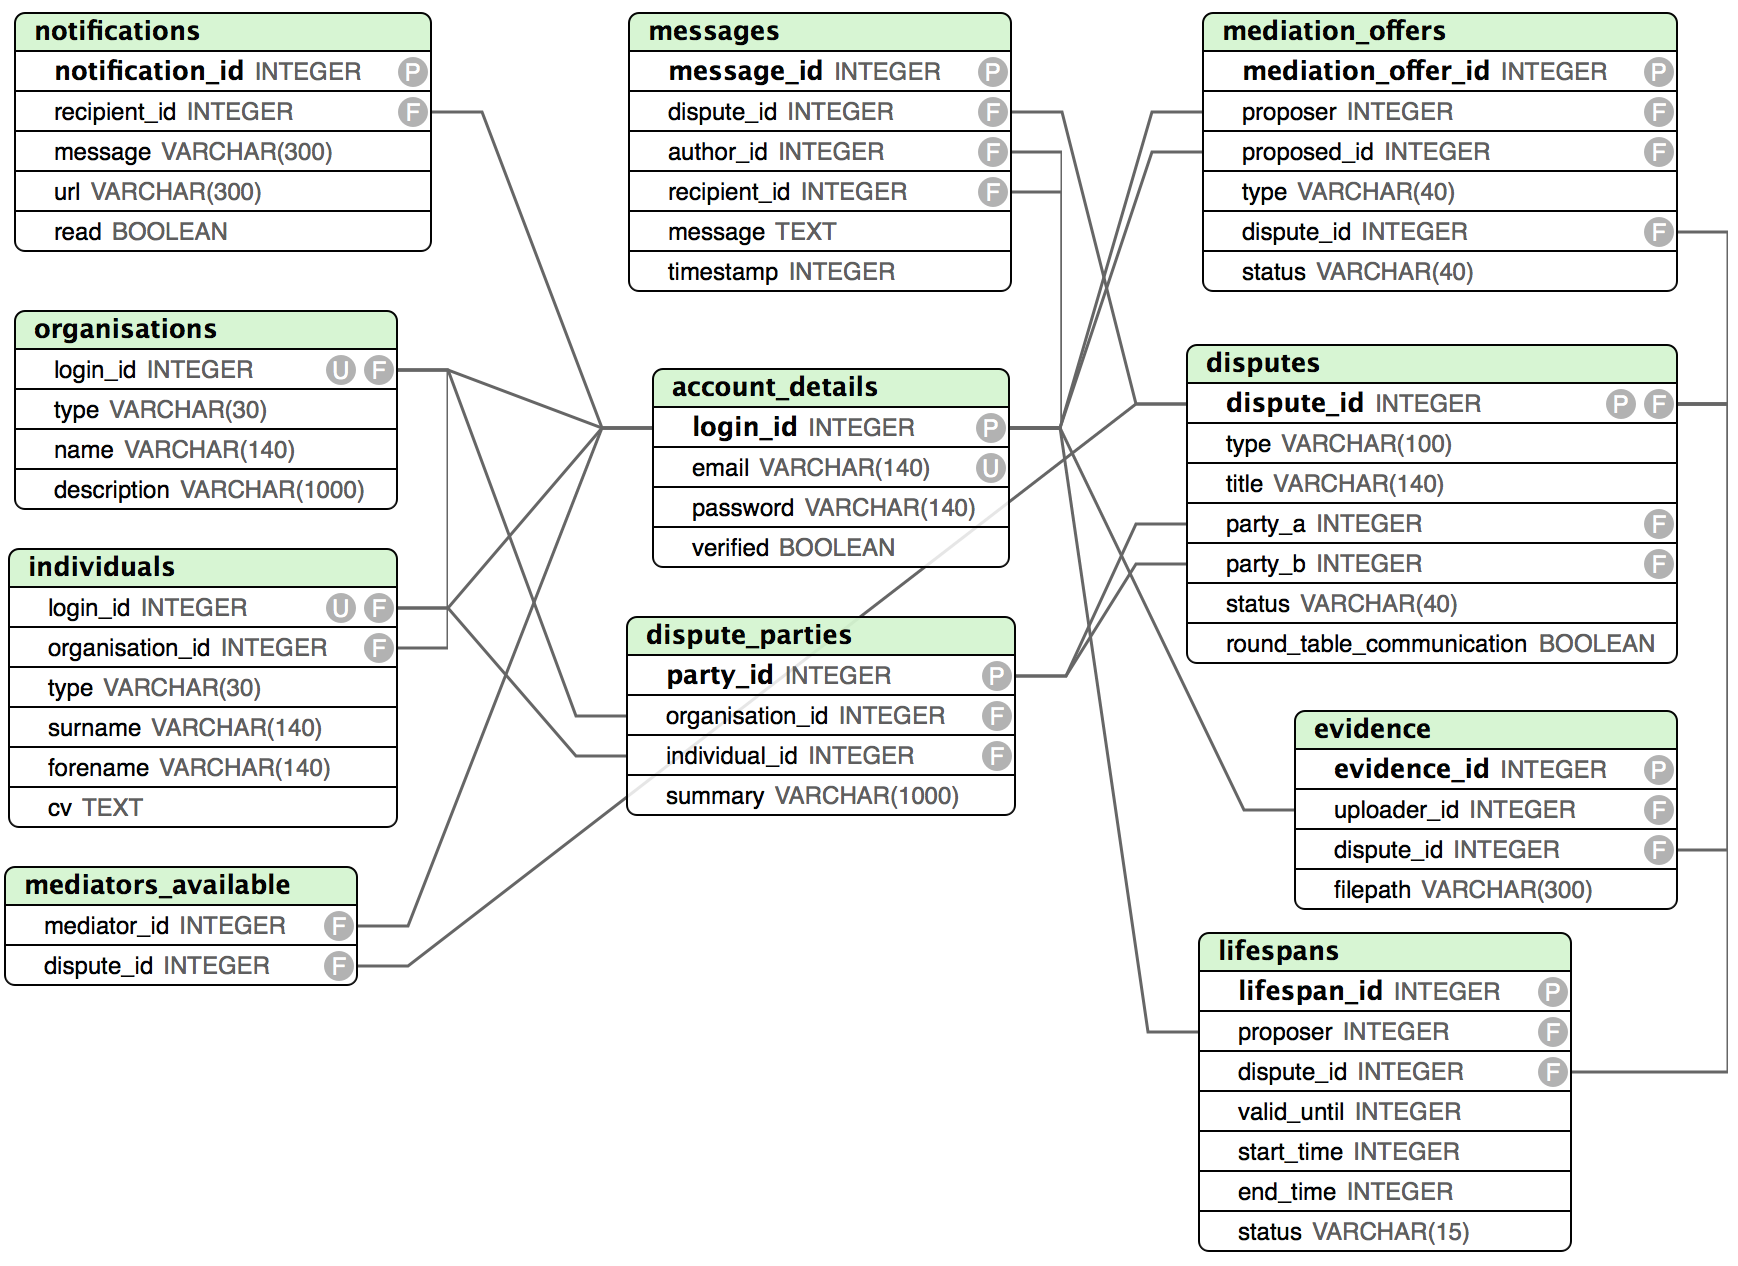
\includegraphics[width=\textwidth]{database}
  \caption{Database schema for the SmartResolution core platform}
  \label{uml:databaseSchema}
\end{figure}

Figure~\ref{uml:databaseSchema} shows the database schema for the SmartResolution core platform, generated directly from \lstinline{data/db.sql} using SQLEditor, for the purposes of this report.

\lstinline{P} symbols refer to primary keys, \lstinline{F} symbols refer to foreign keys, and \lstinline{U} symbols refer to unique integrity constraints. Lines generally denote where one table key references another, i.e. a foreign key visualisation.

For a full explanation and justification of the database design, please refer to appendix~\ref{appendix:database}.

\subsection{Module support}

This section of work is separate from the maritime collision module work, and is concerned with how the core platform should support modules at an abstract level. There should be no maritime-collision-specific code in the core SmartResolution platform, but the platform must support all functionality required by the module.

I took inspiration from WordPress' Plugin API, which uses the concept of 'hooks'. WordPress fires events at various points throughout the normal running of a WordPress installation; these events can be subscribed to and a custom function executed to achieve some arbitrary purpose.

Let us look at the \lstinline{add_filter} function as an example [REF]: %http://codex.wordpress.org/Function_Reference/add_filter

\begin{lstlisting}
add_filter('img_caption_shortcode', 'my_img_caption_shortcode_filter',10);
\end{lstlisting}

The first argument is the event to listen for, the second argument is the custom function to execute, and the third argument is an integer denoting the priority of our subscription (where a higher integer means our custom function is executed before the functions of lower-priority subscribed plugins).

I also wanted to take inspiration from F3's routing API [REF]:

\begin{lstlisting}
$f3->route('GET /some-route' => 'MyClass->handler');
\end{lstlisting}

What I liked about F3's routing is the ability to assign handling to a public method of a class, rather than a global function, keeping the codebase namespaced and tidy.

I used this as a basis for my design:

\begin{lstlisting}
on('event', 'function_to_call', 'priority');
\end{lstlisting}

\subsection{Exposing other methods}

An event-subscription mechanism can only get you so far: I knew I'd need to manipulate the rendered output of SmartResolution, for example adding an item to the dashboard of a dispute.

This could be accomplished by interacting with the core platform, e.g.

\begin{lstlisting}
// @TODO - example code.
\end{lstlisting}

However, this encourages tight coupling between the module and the underlying platform, locking me into a specific design and risking breaking backwards compatibility should I refactor SmartResolution in the future.

Again, I took inspiration from WordPress. WordPress exposes a number of global functions, e.g. \lstinline{get_the_id}, which gets the ID of the current post. [REF] %https://codex.wordpress.org/Function_Reference/get_the_ID

So, I created a number of global functions. [REF] I could now manipulate the rendering of the dashboard like this: % http://smartresolution.org/module-docs/index.html

\begin{lstlisting}
dashboard_add_item(array(
    'title' => 'Some Action',
    'image' => get_module_url() . '/images/icon.png',
    'href'  => get_dispute_url() . '/custom-route'
));
\end{lstlisting}

This is much cleaner and easier from the module developer's perspective. It was always important to me that there should be as few barriers as possible when it comes to module development, if developers are to get excited about SmartResolution.

\subsection{Module persistence}

This was the most difficult area to tackle, as it raises important security issues. Whereas hooking into events and changing the rendering could break aspects of the SmartResolution functionality if the developer is not careful, interacting with the database can do even more damage.

If I allowed arbitrary SQL queries, and a thoughtless developer accidentally executed a \lstinline{DROP TABLE} statement, all manner of data could be lost. This isn't so important on a small demo site with three or four registered users, but if SmartResolution were ever used on a large-scale website, the result could be catastrophic.

Don't get me wrong - you have to trust developers. Regardless of the database access I specifically expose, there's nothing stopping a developer from running PHP's \lstinline{shell_exec} function [REF] and executing any command they wish. And in terms of the database interaction, there's nothing stopping developers from accessing the global \lstinline{DB} object used by the core platform.

My concern was not trusting developers to write perfect code. By allowing module developers to run arbitrary SQL queries, I'm sure most developers would use the ability only for querying the database for a legitimate person. However, if their SQL query takes a user input - for example, if they're writing a search engine module - and they don't sanitise the query, then they're letting the \emph{end user} run arbitrary SQL. And the end user doesn't necessarily have the best interests of SmartResolution at its heart.

I decided to continue with the global function definitions, defining functions supporting specific SQL interactions, e.g. creating tables, selecting rows, updating records, and so on. I toyed with the idea of allowing table schema updates on the fly, creating columns as and when they were needed, but this felt dangerous and was tricky to implement. So I started off proceeding with a \lstinline{declare_table} function:

\begin{lstlisting}
declare_table('my_table', array(
    'a_text_field' => 'TEXT NOT NULL',
    'an_int_field' => 'INTEGER DEFAULT 0',
    'initiated'    => 'BOOLEAN'
));
\end{lstlisting}

This could then be inserted into and queried using specific, named functions. This does somewhat restrict what the developer can do - for example, there is no method for doing SQL table joins - but more often than not, the developer can still achieve what they need to achieve using pure application code.

In the above example, \lstinline{my_table} is not the name of the created table. Instead, it is namespaced as \lstinline{module__[module_name]__my_table}. The module developer doesn't need to know this, and can continue to refer to \lstinline{my_table} in all of their queries as if that is the name of the table.

\section{SmartResolution Marketplace design}

Before I discuss the maritime collision module design, this seems a good place to start, as it follows on from the design for module support rather well.

Early versions of SmartResolution used a PHP array to describe which modules were installed and which were active. [REF] % https://github.com/ChrisBAshton/smartresolution/blob/6287211d49006e87a8d2035906eb58da22217906/webapp/modules/config.php 

What I wanted was an admin dashboard: the ability to sign into an administrator account on your SmartResolution instance, view the installed modules, and activate/deactivate them through a user interface. I also wanted the ability to view modules on SmartResolution.org and download and install them directly through SmartResolution, like WordPress does with plugins.

To accomplish this, I have a JSON feed of featured modules on smartresolution.org. [REF] %http://smartresolution.org/marketplace/feed

This feed is pulled in and converted to HTML, both directly on the marketplace itself [REF] and the SmartResolution admin marketplace dashboard option, emulating what WordPress does with its modules (which are viewable both through your own installation of WordPress and on WordPress itself [REF]). %http://smartresolution.org/marketplace
%https://wordpress.org/plugins/

Defining featured and "other" modules externally on smartresolution.org gives me the freedom to change the contents of that JSON, and therefore change which modules are presented to administrators of SmartResolution instances, regardless of when the instance was installed. This presents a commercial opportunity, as hinted by the "Coming soon" modules for Divorce and Breach of Contract, which I would not offer for free.

The process for putting a module on the SmartResolution Marketplace is currently manual. This is something I would want to automate in the future, for example by taking a GitHub repository URL and zipping up the contents automatically. However, this manual process does at least give me the option to check the code and make sure there is nothing insidious about its contents before making it available on the marketplace.

The admin dashboard feature was one of the last to be added. Figure~\ref{uml:databaseSchema} shows the \lstinline{administrators} table, which requires nothing more than the \lstinline{login_id} associated with an \lstinline{account_details} entry.

Currently, the admin account must be created manually in the database. In future, I would make this a part of the installation process, prompting the user for an admin email and password.

With the admin account created, the admin can log into their account to be presented with three options: Marketplace, Modules and Customise. The latter option is a placeholder and contains no functionality. It is hoped that this might later allow the admin to customise their instance, e.g. by changing the SmartResolution logo, enabling/disabling mediation, and so on.

The other two options are fully functional. The 'Marketplace' converts the modules JSON feed into a HTML page, detects if the module is already installed on the instance, and if not, provides an option to download and install the module in one button press.

The 'Modules' option lists all of the installed modules and whether or not they are active. From this screen, the admin can activate, deactivate or delete the module from their SmartResolution instance.

There is one more admin feature I'd have liked to have added given more time: the ability to switch themes. WordPress allows bloggers to easily change the look and feel of their site by activating a new theme. This is something that is perfectly possible in SmartResolution too, thanks to its MVC architecture.

\section{Maritime collision module design}

The Convention for the Unification of Certain Rules of Law with respect to Collisions between Vessels [REF] describes relatively straightforward, condensed maritime law which can be translated to code. On Dr Constantina Sampani's advice, I used this as the basis for the business logic in my module. %http://www.austlii.edu.au/cgi-bin/sinodisp/au/other/dfat/treaties/1930/14.html

In terms of codifying that business logic, I began by reading the Convention and extracting the relevant questions and conclusions from that. I drew up a data flow diagram to help visualise this: see figure X.

\begin{figure}[h!]
  \centering
    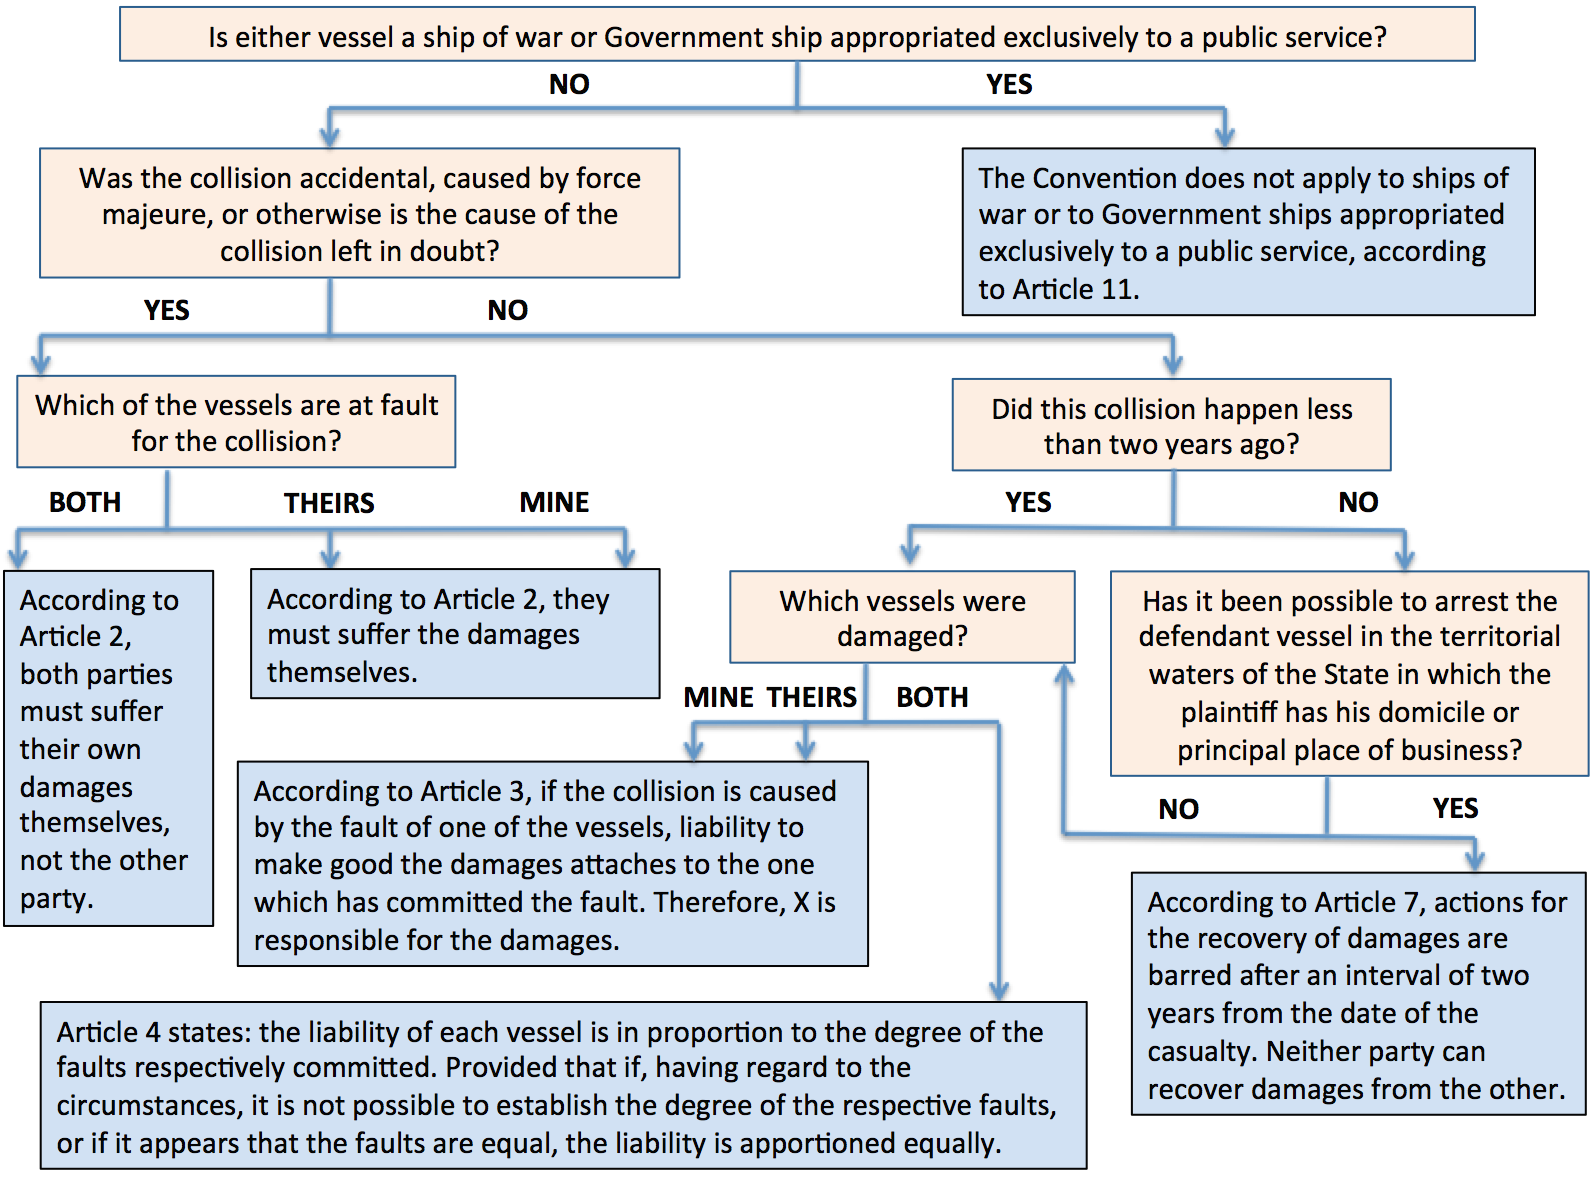
\includegraphics[width=\textwidth]{maritime_collision_logic}
  \caption{Logic for Maritime Law results}
  \label{uml:maritimeLogic}
\end{figure}

Figure~\ref{uml:maritimeLogic}

Certain questions should only be displayed if certain prerequisites are satisfied. I represented the questions as JSON in the following format:

\begin{lstlisting}
    {
        "prerequisites": [
            {
                "question_id":     "article_11",
                "required_answer": "no"
            }
        ],
        "id":   "article_1",
        "text": "Which vessels were damaged?",
        "type": "select",
        "options": [
            {
                "text" : "The vessel of my client",
                "value": "mine"
            },
            {
                "text" : "The vessel of the other party",
                "value": "other"
            },
            {
                "text" : "Both vessels",
                "value": "both"
            }
        ]
    }
\end{lstlisting}

In the above example, the question whose id is \lstinline{article_1} (corresponding to Article 1 of the Convention) is only displayed if the agent answers the question whose id is \lstinline{article_11} with the answer "no".

This module was developed in tandem with the module support in the core platform. As such, it uses most of the events and hooks exposed by the platform.

When the agents have answered all of the relevant questions, the following happens:

\begin{itemize}
    \item The answers are compared to make sure they tally. If one agent says both vessels were damaged and the other agent says only their vessel was damaged, the answers do not correspond and a conclusion cannot be reached. The module cannot be expected to cope with conflicting information. The module would inform the agents of this.
    \item Provided both answers correlate, the module's ResultsCalculator class calls the deduceSummary() method [REF], which contains the hard-coded maritime law logic. A resolution is then presented to the agents.
\end{itemize}

Due to the lack of time the resulting module is a little simplistic, but the point is that the core platform supports any arbitrary module. Modules can be as big and complex as time allows.

\section{User Interface}

I used Bootstrap to set up much of the initial design defaults and as a basis for the layout, wanting a clean and attractive look but not wanting to spend too much time on the user interface. 

SmartResolution should evolve to support the plugging in of different themes. If time allowed, I'd have spent my time implementing that rather than improving the user interface.

That said, I'm pleased with the design and, as I'm using Bootstrap, the theme is fully responsive by default.

\section{Other relevant sections}
\chapter{Implementation} % The implementation should look at any issues you encountered as you tried to implement your design. During the work, you might have found that elements of your design were unnecessary or overly complex; perhaps third party libraries were available that simplified some of the functions that you intended to implement. If things were easier in some areas, then how did you adapt your project to take account of your findings? It is more likely that things were more complex than you first thought. In particular, were there any problems or difficulties that you found during implementation that you had to address? Did such problems simply delay you or were they more significant? You can conclude this section by reviewing the end of the implementation stage against the planned requirements.

\section{Comments}

@TODO mention this somewhere:

The codebase is liberally commented throughout, using API-style markup. This was a difficult decision, discussed and justified in appendix~\ref{appendix:comments}.

\section{SmartResolution directory structure}

As the implementation followed an agile methodology, the design evolved over time and thus, the directory structure could not be determined up-front. Most (but not all) of the key directories and folders are outlined below:

\begin{samepage}
\dirtree{%
.1 data/.
.1 features/.
.1 test/.
.1 vendor/.
.1 webapp/.
.2 core/.
.3 api/.
.3 controller/.
.3 db/.
.3 model/.
.3 view/.
.2 modules/.
.3 other/.
.3 config.json.
.2 uploads/.
.2 index.php.
.2 routes.php.
.1 .travis.yml.
.1 composer.json.
.1 Gemfile.
}
\end{samepage}

\lstinline{data} contains fixture data for tests. This is also where the test and production SQLite3 databases reside.

\lstinline{features} contains the Cucumber features and Ruby step definitions.

\lstinline{test} contains all PHP unit tests.

\lstinline{vendor} is an automatically generated directory, created by Composer, containing all of SmartResolution's dependencies.

\lstinline{webapp/core} contains the core ODR platform, which uses an MVCR compound design pattern (\lstinline{webapp/routes.php} defines the routing component). The \lstinline{model}, \lstinline{view} and \lstinline{controller} directories are self-explanatory.

Also inside the core is the \lstinline{db} directory, which contains middleware classes connecting the model classes to the database, since models should encapsulate the concept of whatever it is they are representing, rather than being responsible for the relational database to object mapping.

Finally, this folder also contains an \lstinline{api} directory, which defines all of the global functions available to modules. Having these in their own directory made generating module-specific API documentation easy.

Going back up a level, we have \lstinline{webapp/modules}, which contains any installed SmartResolution modules. This is where the maritime collision module resides once it has been installed. A \lstinline{config.json} file (edited in a user-friendly way through the admin dashboard) denotes which modules are installed and whether or not they are active.

Finally, at the top level we have a few interesting files:

\lstinline{.travis.yml} - an instructions file for Travis Continuous Integration, describing how to set up the project and run its tests.

\lstinline{composer.json} - describes SmartResolution's dependencies. Developers can install all dependencies simply by running \lstinline{\$ composer install}.

\lstinline{Gemfile} - describes SmartResolution's Ruby dependencies. Required for the Cucumber and Ruby integration tests.
\chapter{Testing}

SmartResolution is an open-source platform being marketed to those wanting to provide ODR services, and as such it is very important that the platform itself is thoroughly tested. Subscribers need to have confidence that the core platform works as it should, and module developers need to have confidence that the underlying system is robust enough to support their module. For these reasons, the core platform implementation was done alongside unit and integration tests throughout.

In an ideal world, the same principles would have been applied to the Maritime Collision module and to the SmartResolution website and marketplace. However, developing the core platform in a test-driven way turned out to be quite a slow, methodical process - read more in the evaluation section - and I felt that doing the same for the lesser two components was a luxury I could not afford with an impeding deadline. Therefore, this section is mostly concerned with testing the core SmartResolution software.

As previously mentioned, the project was developed in an agile way from mid-way through the design stage onwards. As such, the principles of business-driven development (BDD) and continuous integration (CI) were applied throughout the implementation. This section discusses the testing strategy that was applied during the implementation.

\section{BDD}

The project was developed in a business-driven way, as demonstrated in figure~\ref{uml:bdd}.

\begin{figure}[h!]
  \centering
    \ifimages
    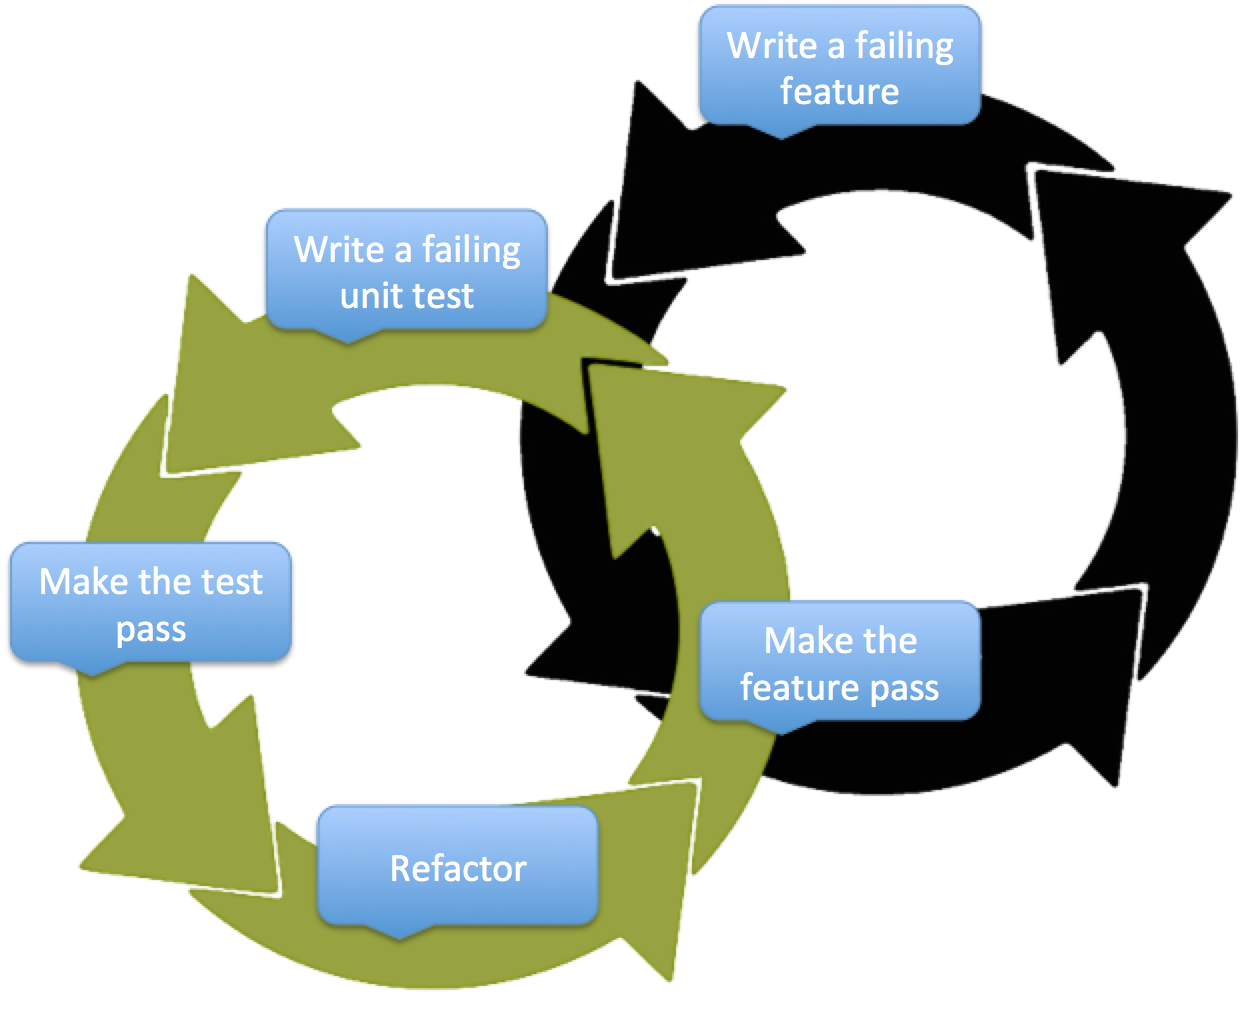
\includegraphics[width=\textwidth]{bdd}
    \fi
  \caption{The BDD development process: an extension of TDD}
  \label{uml:bdd}
\end{figure}

To begin with, a Cucumber feature is selected and executed. It should fail. Now a unit test is written to describe a low-level implementation of the feature. The unit test is run and again it should fail. The next step is to write the simplest code possible to make the unit test pass.

With the test passing, now is the opportunity to take a step back and look at the code in the context of the codebase as a whole. Can anything be refactored? If so, apply the refactoring step, then run the unit tests again to ensure that everything still works as correctly.

The unit-test process outlined above is known as the ``red, green, refactor" workflow and is repeated over and over until we have enough of the feature implemented to make a step of the feature pass, and then another step, and so on, until the feature as a whole is completed and passes the integration test.

Occasionally, features were too cumbersome to implement in a BDD manner, as they required spanning multiple architectures (routing, database layers, models, controllers, and so on). Wherever following BDD wasn't appropriate, I added unit and end-to-end tests post-implementation.

\section{Test database}

Cucumber regression tests are end-to-end and use a headless browser to emulate the browser environment, clicking buttons and filling in forms, then querying the state of the HTML to validate that an element of functionality worked as expected.

To accomplish this, the driver (in our case, Poltergeist) accesses the server like a normal browser. However, our tests rely on the database having certain fixture-data and will also be making persistent changes to the database, so it's essential that the tests use a test database, rather than the production database.

Poltergeist allows you to override the HTTP headers sent with each request, so my Cucumber tests modify the User-Agent property to be either \lstinline{Poltergeist} or \lstinline{Poltergeist--clear}. Both headers inform the application that it should use the test database, but the latter provides an additional instruction that the database should be cleared and re-populated with test data before processing the request. This is demonstrated in figure~\ref{uml:headers}.

\begin{figure}[h!]
  \centering
    \ifimages
    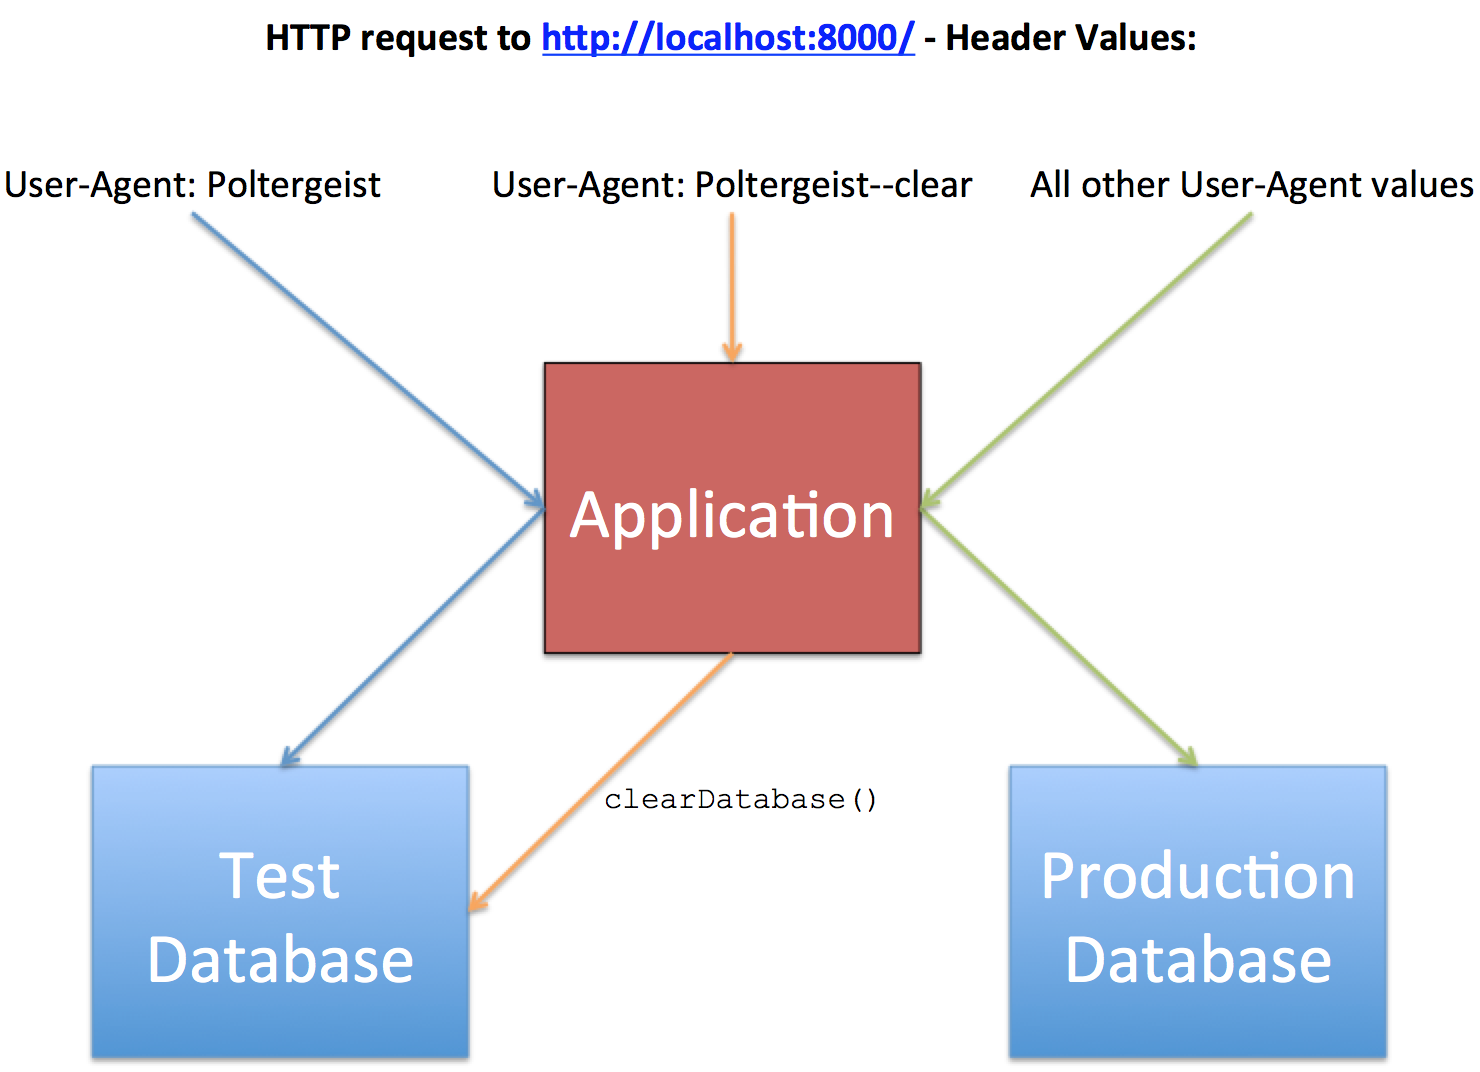
\includegraphics[width=\textwidth]{headers}
    \fi
  \caption{Visualisation of how SmartResolution determines which database to use depending on the received HTTP headers}
  \label{uml:headers}
\end{figure}

There's nothing stopping the end-user changing the headers that they send, so they too could access SmartResolution and interact with the test environment rather than the production environment. Ultimately, this is completely harmless. The test database is cleaned every time the test suite is run, so they would not even be able to sabotage the tests. This is a tried and tested technique, and has been adopted by companies including the BBC~\cite{bbc:cucumber}.

\section{Unit Testing}

Almost every class in the system has an associated unit test. This does not apply to library classes, such as those provided by F3, since the responsibility for testing those classes resides with the third party. Unit tests verify that the publicly available methods of a class work as expected, both when accessed correctly and incorrectly.

The nature of unit tests should be that they are loaded into memory and are very quick to run. ``Depending on your platform, your testing tool should be able to run at least 100 unit tests per second."~\cite{artOfAgile} True unit tests are also entirely self-contained. According to Michael Feathers, a ``test is not a unit test if it talks to the database, it communicates across the network, it touches the file system or it can't run at the same time as any of your other unit tests.''~\cite{feathers:unitTests}

Some of the unit tests in SmartResolution are not `true' unit tests, as they rely on a database connection and the existence of specific fixture data. Additionally, some unit tests might alter, add or remove items from the database.

Towards the end of the project I refactored my tests to cut down on the number of unit tests that were tightly coupled to the database: this is discussed later on in this section. Until then, I'll discuss my testing strategy from the mindset I held at the beginning of the project, which was that code coverage is the most important metric, not test speed.

\subsection{Database transaction threads}

\subsubsection{Database transactions and PHP}

Often, we want to accomplish several things in one `transaction', for example, debiting one person's account and crediting the other person's account. If the debiting of the first person's account fails - for example, if doing so would make their account balance negative - then we don't want the other person's account to be credited. Both queries must happen, or neither must happen.

Transactions are supported in PDO (PHP Data Objects) and in F3's wrapper for PDO, where we are able to define the start and end points of a transaction. The above example could be represented in code as follows, and if either query in the transaction fails, neither would be applied:

\begin{lstlisting}[language=php]
$db->begin();
$acc1->debit(400);
$acc2->credit(400);
$db->commit();
\end{lstlisting}

\subsubsection{Issues with testing database transactions}

Between test suites, SmartResolution runs the `clear database' command to revert the test database to a known constant: an untainted database filled with predefined fixture data. This reverses any changes that may have been made to the database when running the previous test suite.

This is a useful technique in ensuring that test suites don't corrupt one another's results and that each suite works with the same set of data. However, it is slow and takes around a second on a reasonably powerful machine, becoming a problem if the script is called too often.

I made a conscious effort to keep these resets to a minimum, but a problem I faced early on in my unit tests was the following error message:

\begin{lstlisting}
PDOException: There is already an active transaction!
\end{lstlisting}

The exception refers to a situation in database transactions whereby a transaction was initiated, perhaps some queries were queued for the transaction, and then there was another request to begin a transaction. Somewhere in SmartResolution, a transaction was not being committed or rolled back.

This exception was usually raised after testing a part of my application that should (and does) raise an exception, such as trying to assign a law firm as the agent of a dispute. The expected exception was being raised and that was preventing the change (the assignment of the law firm to the dispute) from being made persistent, but subsequent attempts to begin new transactions complained that a transaction was already in progress.

Early on, this wasn't too much of an issue: I was able to run the `clear database' command between any unit tests that raised this exception, as removing and re-creating the database would naturally clear any outstanding transactions. This was a bit of a hack, but felt justified as the test and production environments are very different. In the test environment, hundreds of transactions are initiated when running the unit tests and all tests are hooking into the same database connection. In the production environment this would not happen: if an exception is raised, an error page is triggered and the user is faced with an error message relating to the exception. Once PHP delivers the error page to the user's browser, the database connection is no longer open and thus a new transaction can begin.

For several weeks, I was happy with this solution, but it did mean that my tests were quite slow to run. You can see in a Travis build around that time that it took almost a minute to run 90 unit tests\footnote{A build on 15th April, before refactor: \url{https://travis-ci.org/ChrisBAshton/smartresolution/builds/58603809}}, violating James Shore's principle that unit tests should run almost instantly.

Eventually, I decided to spend some time investigating the issue. I deduced that the transaction was not being committed because an exception was being raised before it could be committed. What I did not realise was that transactions were not being automatically rolled back when an exception was raised - it was something that needed to be handled manually in each exception.

Handling the transaction rollback in each raised exception would mean writing code like this:

\begin{minipage}{\textwidth}
\begin{lstlisting}[language=php]
$db->begin();

// several lines of code and database queries

if (// some condition) {
    $db->rollback();
    throw new Exception('Error!');
}

// more lines of code and database queries

if (// another condition) {
    $db->rollback();
    throw new Exception('Another error!');
}

$db->commit();
\end{lstlisting}
\end{minipage}

This seemed laborious, error-prone and messy. Instead, I defined a custom exception function which throws an exception, but also rolls back any existing transactions.

\begin{minipage}{\textwidth}
\begin{lstlisting}[language=php]
    public function throwException($message) {
        try {
            Database::instance()->rollback();
        } catch (Exception $PDOException) {
            // do nothing - we only wanted to roll back the transaction if one existed.
            // since one doesn't exist, there's nothing to roll back. Let's just continue and
            // throw the Exception we wanted to throw in the first place.
        }
        throw new Exception($message);
    }
\end{lstlisting}
\end{minipage}

Now that the root of the problem had been fixed, unit tests could be run without clearing the database in between each test. This led to big improvements in test speed: at this stage, I could now run 112 unit tests in 34 seconds.\footnote{A build on 17th April, after refactor: \url{https://travis-ci.org/ChrisBAshton/smartresolution/builds/58932345}} This is 3.29 unit tests per second (UTPS), compared with 1.58 UTPS before the optimisation.

I still needed to clear the database between each test \emph{suite}, as the tests would still alter the state of the database. But now, by and large, most of the tests \emph{within} those suites did not need to run on a new database connection.

\subsection{Refactoring to pure unit tests}

Earlier I described how `pure' unit tests should not query a database. An unfortunate consequence of the implementation of my code was that database querying was essential to unit test my classes, as my models were populated by an ID representing a row in the database, rather than populated with an array of data which may or may not have come from a database.

For example, the \lstinline{Message} class expected to be passed an ID to its constructor. Inside the constructor, a function call was made to a data wrapper class which contained the business logic for retrieving from the database the class-specific data (such as message content, author ID, etc) corresponding to the given ID. The returned array was then used to populate the model. This somewhat decoupled the model from the database - all SQL queries were encapsulated in the intermediary database querying objects - however, it made the models quite difficult and slow to test.

The decision to implement the models like this was to make life easier for the controllers. Let us examine this with some pseudo-code:

\begin{lstlisting}[language=php]
// inside a controller
$disputeID = getDisputeIDFromUrl();
$dispute = new Dispute($disputeID);
\end{lstlisting}

Inside the Dispute model, we had something like this:

\begin{minipage}{\textwidth}
\begin{lstlisting}[language=php]
function __construct($disputeID) {
    $disputeDetails = DisputeDatabaseConnector::getDisputeDetails($disputeID);
    $this->title = $disputeDetails['title'];
    // and so on
}
\end{lstlisting}
\end{minipage}

Though the model was made a little impure due to the database connection object, I could write nice code in the controllers that only had to worry about getting an object's ID. This meant that I could chain method calls together, passing returned IDs into subsequent constructors to quickly and easily get the objects I needed.

\subsubsection{Refactored solution}

Refactoring constructors to take arrays of data rather than IDs took some significant effort and meant extracting the database querying out of the models:

\begin{lstlisting}[language=php]
// inside the Dispute model
function __construct($disputeDetails) {
    $this->title = $disputeDetails['title'];
    // and so on
}
\end{lstlisting}

The database query instead had to be moved to the controller;

\begin{lstlisting}[language=php]
$disputeID = getDisputeIDFromUrl();
$disputeDetails = DisputeDatabaseConnector::getDisputeDetails($disputeID);
$dispute = new Dispute($disputeDetails);
\end{lstlisting}

The advantage of the refactored solution is that the models become pure: they now have no concept of a persistence layer. We can now test our models by passing arrays of hard-coded data, removing the need to retrieve from and write to a database.

Changing object constructors to take arrays rather than database record IDs meant I could cut down test times significantly. After implementing the refactored solution, my test suite performed 109 unit tests in just 12.7 seconds: a UTPS of 8.57.\footnote{A build on 22nd April, after final refactor: \url{https://travis-ci.org/ChrisBAshton/smartresolution/builds/59532839}} This information is summarised in comparison table~\ref{table:testTimes}. It is worth noting that those are the results on Travis: on my MacBook Pro, the entire unit test suite runs in under six seconds.

\begin{table}[h!]
\label{table:testTimes}
\begin{center}
\begin{tabular}{ l | r | r | r | r | r}
  Stage in project & Unit tests & Assertions & Time taken (s) & UTPS & APS \\
  \hline
  Pre-refactor & 90 & 221 & 57.70 & 1.58 & 3.83\\
  Fixed database transactions & 112 & 263 & 34.24 & 3.29 & 7.68\\
  Refactored to use only pure models & 109 & 309 & 12.72 & 8.57 & 24.29
\end{tabular}
\end{center}
\caption {Table showing the unit test times after various refactoring steps}
\end{table}

\subsubsection{Further refactoring}

Extracting the database retrieval out of the model also meant extracting the database \emph{changes} out of the model. I took the opportunity to refactor this behaviour too.

Beforehand, I had code like this inside my models:

\begin{lstlisting}[language=php]
// inside the Dispute model
function closeSuccessfully) {
    SomeDatabaseConnector::updateField('disputes', 'status', 'resolved', $this->disputeID);
}
\end{lstlisting}

This was tightly coupled to the underlying table representation, and became fiddly when having multiple functions that change different fields. When moving this behaviour into the controllers, I decided to encapsulate all updates inside one update method that corresponds to the model:

\begin{lstlisting}[language=php]
// inside the Dispute controller
$dispute->closeSuccessfully();
$update->dispute($dispute);
\end{lstlisting}

Instead of updating an individual field value, I now pass the entire Dispute object to an update method which knows how to map the dispute object to its representation in the database. It calls the necessary methods on the dispute object (such as \lstinline{$dispute->getStatus()}) to collect all of the information it requires to update the record.

This large refactoring task perhaps hints at a broader problem: object-relational mapping. It could be argued that at various points in my codebase I have not approached the problem in the object-oriented way I should have, because I've had to manually map the object to be in terms of its underlying relational database representation. Perhaps, in hindsight, an object-relational database would have been more appropriate than an RDBMS, to delegate the understanding of the object-relational mapping to a third-party.

\section{Functional Testing}

The SmartResolution core software is described through a collection of Cucumber features, associated with step definitions. These features are executable and can automatically verify that the system is working as expected. As a reminder, the full list of tested features is outlined in appendix~\ref{appendix:requirements}, and the justification for the choice of Ruby and Cucumber as the BDD framework is in appendix~\ref{appendix:bdd}.

\subsection{Functional tests structure}

Every Cucumber feature has a corresponding step definition, defined in a step definition file of the same name as the feature. Each step definition defines a step in a Cucumber scenario in terms of interacting with the page, through methods provided by the Capybara acceptance test framework. Capybara requires a browser driver such as Poltergeist to request and then render the webpage. The browser can be headless (running as a background process, hidden from view) or a window browser. Poltergeist, as the name might suggest, is headless.

In cases where step definitions were beginning to rely on methods defined in other step files, I extracted the methods out as a common helper class. For example, step definitions have access to a `Session' helper class which provides methods to log in with specific credentials, or log into account types (e.g. \lstinline{Session.login_as_agent}). Figure~\ref{uml:cucumber} demonstrates the relationship between a Cucumber feature, its step definition, and the helper classes.

\begin{figure}[h!]
  \centering
    \ifimages
    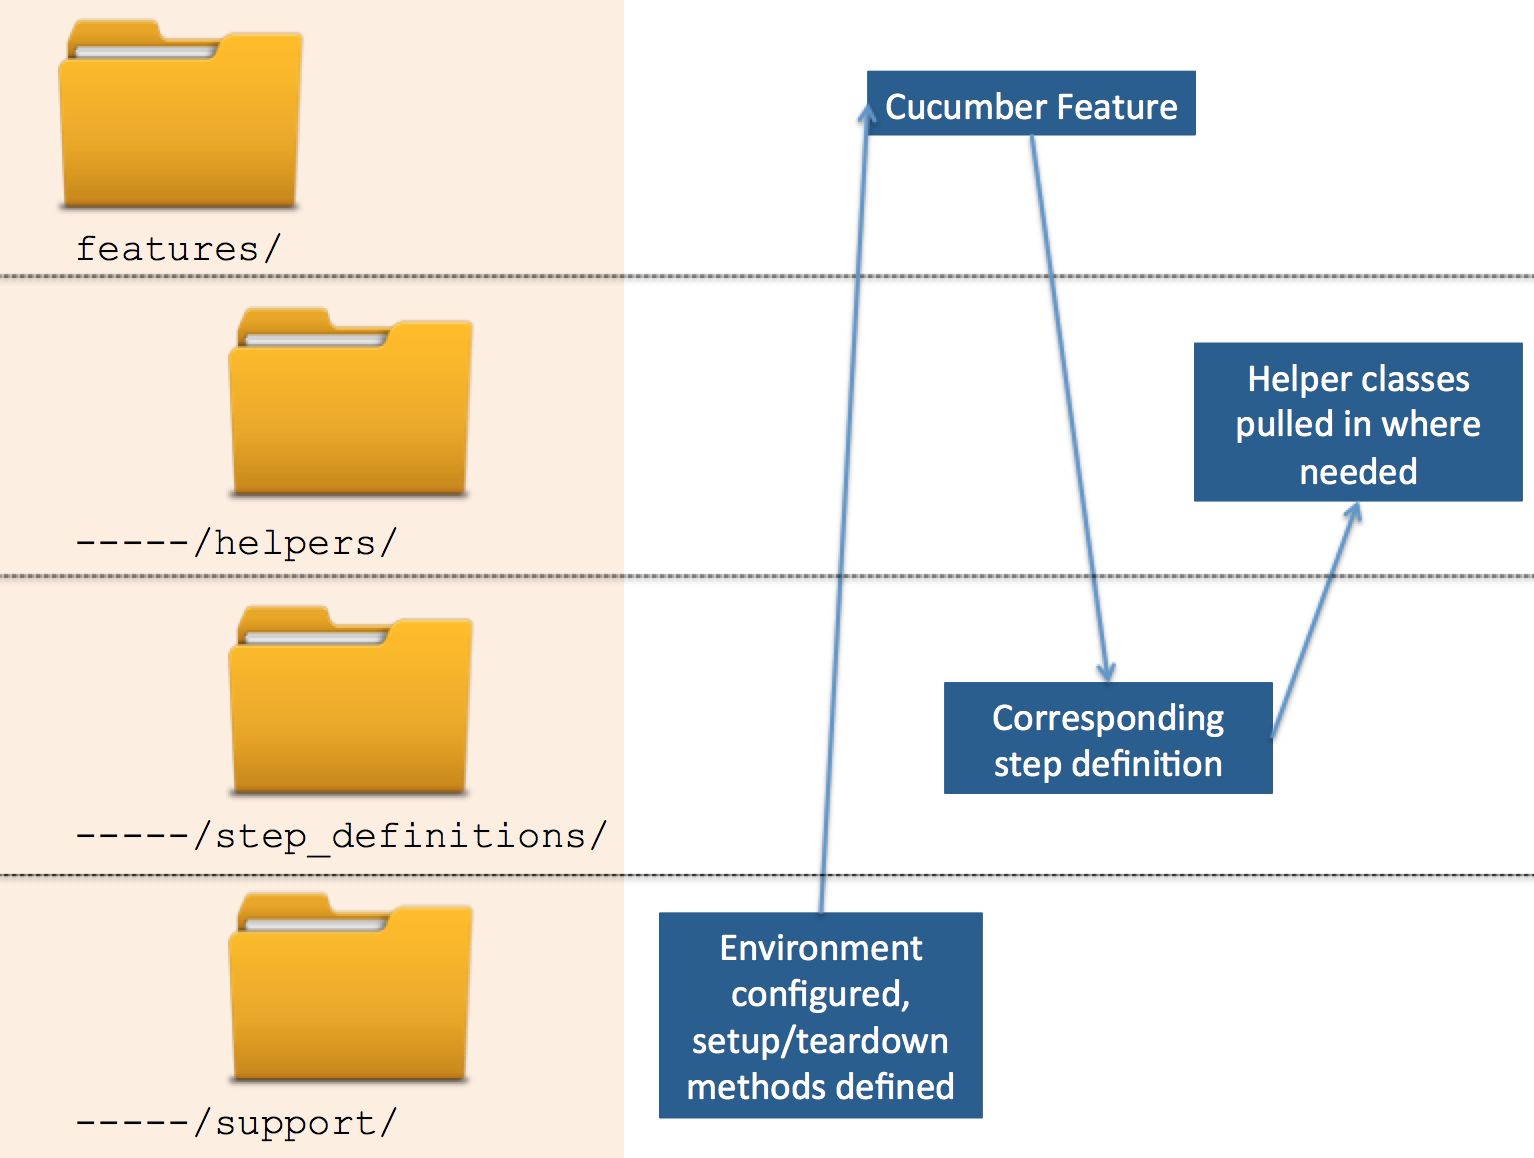
\includegraphics[width=\textwidth]{cucumber}
    \fi
  \caption{Visualisation of which files are involved in defining a Cucumber feature}
  \label{uml:cucumber}
\end{figure}

Finally, there are also numerous steps which are repeated across different features, such as ``Given I am logged into an Agent account". In cases such as these, it became difficult to maintain those step definitions when it could have been buried in any of the step definition files whose features depend on it, so these were extracted to a `\_common.rb' step definition file. This is now the first place one should look when trying to find and maintain a step definition.

\subsection{Database-clearance optimisation}

The process of clearing the database involves removing the SQLite database entirely, creating a new SQLite database, executing the table-setup SQL (all performed via shell commands through PHP's \lstinline{shell_exec} function) and then seeding the database with fixture data. This fixture data is defined in \lstinline{data/fixtures/fixture_data.yml} and the mapping of YAML data to SQL tables is defined in \lstinline{data/fixtures/seed.php}. As already mentioned, this is quite a slow process and takes around a second even on a powerful machine.

I refactored my unit tests to cut down the number of `clear database' instructions, but this was an optimisation I had in mind from the start when it came to my Cucumber features. Unlike unit tests, Cucumber features test the system from the user's perspective and by their very nature require interaction with the database. The database needs clearing and re-populating between some tests to prevent the actions of one test from corrupting the other, ensuring that every test has access to the same data.

I kept the number of `clear database' instructions to a minimum in my Cucumber tests by annotating specific features with the \lstinline{@clear} tag to indicate that the database should be cleared before executing that feature. Any features without that tag are less likely to be testing something that makes persistent changes. The inclusion of the \lstinline{@clear} tag tells Poltergeist to send the \lstinline{Poltergeist--clear} header rather than just the \lstinline{Poltergeist} header.

\subsection{A note on feature style}

There is a trade-off between having a verbose Cucumber feature and a verbose step-definition. The former bogs the feature down in detail and risks devaluing it, whereas the latter can make maintenance more difficult.

I argued this same internal battle in the \emph{Developing Internet-Based Applications} assignment, discussing the pros and cons of each in some detail. The relevant extract of that report is included here in appendix~\ref{appendix:cucumber}.

My conclusion was that, though the two need to be balanced, it isn't detrimental to specify specific fields and error messages in the Cucumber feature itself. The alternative - abstracting that information away in the step definition - can make it difficult to maintain state throughout the scenario. Following this conclusion, some of the Cucumber features decided upon in the initial requirements were later reworded to fit in with this philosophy, though their purpose and relevance remained the same.

For example, this was an original `lifespan negotiation' scenario:

\begin{lstlisting}
  Scenario: Accepting a Dispute lifespan offer
    Given the other Agent has sent me a Dispute lifespan offer
    Then I should be able to accept the offer
    And the Dispute should start
\end{lstlisting}

This is how the scenario looks now that the step definitions have been implemented:

\begin{lstlisting}
  Scenario: Accepting a Dispute lifespan offer
    Given the other Agent has sent me a Dispute lifespan offer
    Then I should be able to Accept the offer
    And I should see the message 'Dispute starts in'
\end{lstlisting}

The original and amended scenarios are very similar, but the latter is a little more tied to the implementation. The `I should see the message' step definition is reused across many scenarios and means that the step definitions as a whole are simpler and cleaner, even if the Cucumber features themselves are slightly more verbose than before.

\section{Continuous Integration}

Travis CI ran all unit and functional tests on every pushed commit or pull request, automatically notifying via email if anything broke. It was an invaluable tool throughout the project and was well worth spending time configuring.

The most difficult aspect to setting up Travis was getting the PHP server running, since Travis only supports one terminal window. The PHP server had to be set up as a background process so that Travis could continue to run the other commands required to run the tests.

Travis wasn't the only tool that performed a service on every pushed commit. Just as important as ensuring that all tests continue to pass is ensuring that dependencies remain up-to-date. Gemnasium periodically checks the status of SmartResolution's dependencies and warns via the embedded SVG in the project README whether or not a newer version is available.

Dependency tracking is important, as newer versions of dependencies fix bugs and vulnerabilities discovered in older versions. By not updating SmartResolution's dependencies regularly I would risk crackers being able to exploit unpatched vulnerabilities. This is especially relevant since SmartResolution is open-source and anybody can see which version of which third-party library SmartResolution is using.

Another important thing to monitor with each commit is code quality, something that CodeClimate is trying to automate. Whenever I push a commit to SmartResolution, CodeClimate queues another scan of the codebase and informs me on a level of 1-4 whether the quality of my codebase has improved or deteriorated, using metrics such as variable name length, code duplication, the number of possible paths through a block of code, and so on. Utilising this third-party service helped fight the temptation to hack a bit of functionality in, instead encouraging good engineering practice and providing suggestions as to how the codebase could be made more maintainable.

\section{User Testing}

Whereas it is the software engineer's responsibility to ensure that the project is built right, it is the customer's responsibility to ensure that the right project is built. Therefore, user testing with the customer is critical.

As has already been highlighted, the customer for this project was extremely busy and was unable to meet more than a couple of times. This made user-testing very difficult, but I tried my best to offer alternative options.

It was good that I spent so long clarifying requirements at the beginning of the project. In the absence of regular communication and feedback, this original set of features was invaluable in ensuring that the system contained all of the required functionality.

Mid-way through the project, I deployed SmartResolution to smartresolution.org and invited all stakeholders to try out a beta version of the project, describing how to log into the system, what functionality had already been implemented, and what functionality had yet to be implemented.

Throughout development I adhered to the agile principle of regular releases, pushing the latest stable version of SmartResolution to the website on a daily basis so that the customer would be able to feel the benefit and experience a more feature-complete demo.

Later on in the project I made it even easier to demo the software, by producing a short video demonstrating the software and the maritime collision module. This is embedded on the homepage of smartresolution.org and enables users to see what the system is capable of without having to manually log in and out of demo accounts representing different user roles.

Where feedback was lacking from the customer, I turned to friends, family and the Twitter community to try out the demo and give me constructive comments to work on. These comments were fed back directly into my design, leading to the following improvements:

\begin{itemize}
\item Smaller icons. My early designs used dashboard icons around 3 times larger than the final design. I was trying to emulate clear and minimalist dashboards such as the one on DigitalOcean (see figure~\ref{screenshot:digitalOcean}) but my implementation was something consistently questioned in the feedback I received.
\item Larger font size. Bootstrap's default font was too small given the sparseness of the design as a whole. I increased the base font size; all font sizes across the site increased in size proportionally, as my CSS defined fonts in terms of \lstinline{em}.
\item Responsive improvements. It was never a requirement to make the SmartResolution software fully responsive: the fact that Bootstrap supports responsiveness by default was just an added bonus. However, some of my design decisions - such as absolutely positioning the lifespan status at the right hand side of the dispute - made for a poor experience on mobile. When this was pointed out in the feedback, I added a media query so that the positioning would only apply on devices of a minimum screen width.
\end{itemize}

\begin{figure}[h!]
  \centering
    \ifimages
    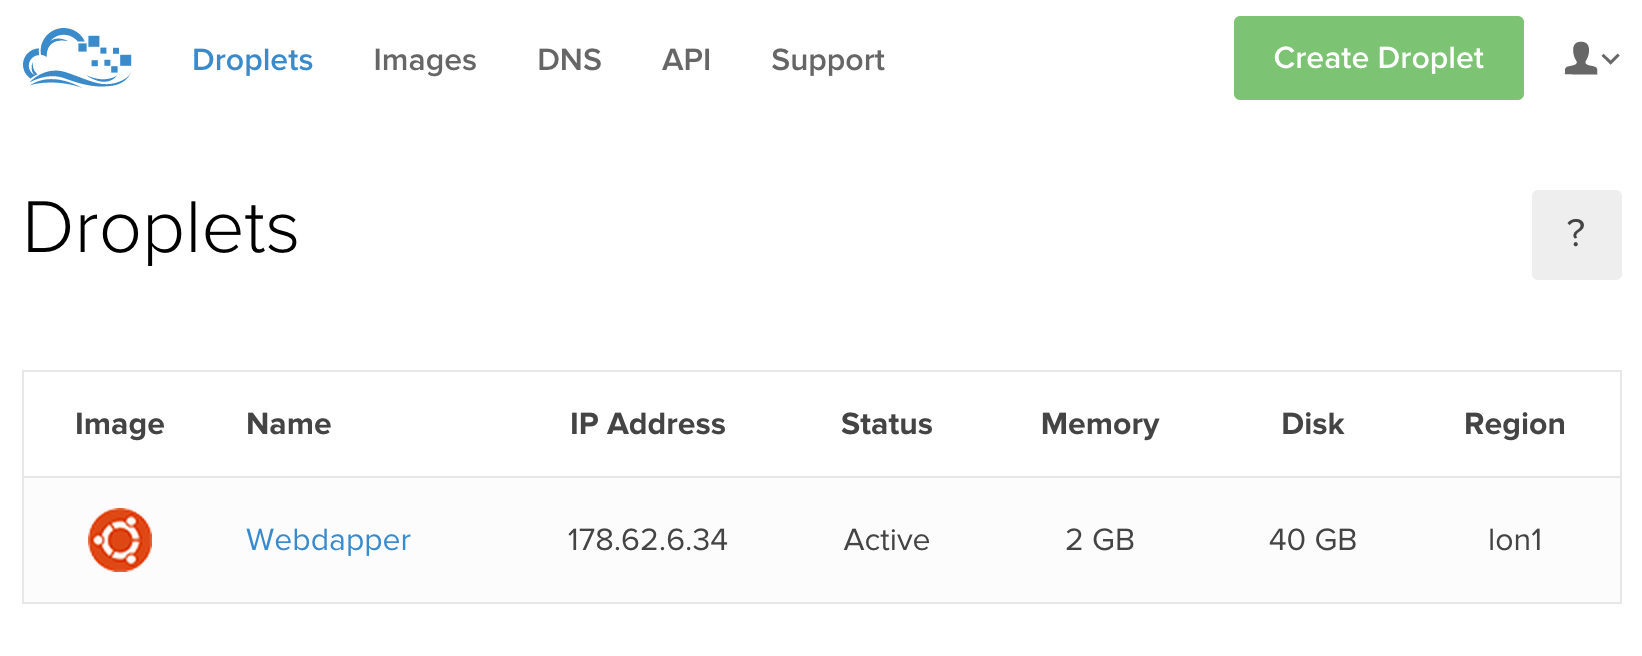
\includegraphics[width=\textwidth]{digitalocean}
    \fi
  \caption{Screenshot of the clean and simple DigitalOcean interface I wanted to emulate in the design for SmartResolution}
  \label{screenshot:digitalOcean}
\end{figure}

Feedback regarding the workflow of a dispute had to be treated differently, since the customer was the law expert and the people giving feedback were not law experts. However, their comments were collected and fed back to the law expert for trying to negotiate simpler dispute workflows.

One of the original requirements was for a formal resolution-offering process. An agent would be able to make an offer by filling in a HTML form denoting offer details, damages awarded, and so on. I was able to simplify this in light of the feedback: agents are human beings and can reach that kind of resolution through the communication option alone. They can then close the dispute successfully, with no need to officially form a structured offer that SmartResolution understands. Removing these artificial constraints made for a more user-friendly workflow and reduced the development overheads significantly.
\chapter{Evaluation}

\section{Were the requirements met?}

As a reminder, the original requirements were identified as the following, to be tackled iteratively:

\begin{enumerate}

    \item Find or build an Online Dispute Resolution platform
    
    \item Tailor the platform towards maritime collision disputes

    \item Make the platform abstract, able to take a module of business logic
    
    \item The maritime collision module should be able to retrieve the most similar historical cases

    \item The details of these historical cases should be fed back into the details of the current dispute, thereby influencing the court simulation

\end{enumerate}

The scope of these deliverables could have been different had there been an existing ODR platform which I could use as a basis for the project. The fact that the platform had to be designed and developed from scratch was a considerable burden on time and resources, even before applying the concepts of extending the platform and developing a maritime collision module for it.

The first three of these were the core requirements, but I distinctly remember that the fourth and fifth requirements were my own idea. The thought of making use of historical maritime collision cases excited me at the time and felt like a logical progression for the module. Both my supervisor and the client were happy to agree to make this a part of the requirements specification.

Over the course of the project, I was able to look beyond the specialised area of maritime law. The light bulb moment came when I considered the commercial viability of the project (see appendix~\ref{appendix:commercialViability}), particularly the comparison with WordPress' commercial model. It was then that I saw the big picture and realised that the success of the platform would depend entirely on its extensibility, its ease of use, its ease of development and its branding.

\subsection{Prioritising the components}

Whereas the first three requirements remained, the fourth and fifth requirements took a back seat whilst I developed the SmartResolution website (alongside the continuous deployment script), the SmartResolution Marketplace, the admin dashboard facility and the detailed documentation for module developers. It could be argued that the first three of the original requirements were correctly identified and delivered, whereas the remaining two were surpassed by more pressing and relevant requirements, which were also subsequently delivered.

I wanted to create something that could be physically used in the real world at the end of my project and tried to see the big picture at all times. The big picture is a robust and fully extensible core ODR platform supporting an infinite number of modules that can be developed to fulfil an infinite number of uses.

It was important that the core platform offered enough hooks and an expansive-enough API to allow for the requirements we haven't even considered yet. It was equally important that there should be a straightforward way to install said modules into one's installation of the SmartResolution software. At this stage I took further inspiration from WordPress and decided to create an embedded marketplace, accessible from within the software but referencing an external site. This allows me to update the list of available modules independent of when a SmartResolution instance was installed and what version it might be.

If I had foregone the SmartResolution marketplace component entirely, I could have invested around a fortnight of extra development time in the maritime collision module, and perhaps accomplished something more exciting and groundbreaking in the AI. However, without a centralised means of browsing and installing modules, and indeed a centralised means of downloading the core platform itself, then this may very well have died off as a forgotten university project. I like to think that, with the platform built and the documentation plentiful, developers are empowered to develop their own modules for this sector which has recently been gaining in popularity and public awareness.

In essence, the minimum requirements were a working ODR platform and a maritime collision module prototype. Anything beyond that in terms of delivery was my own prerogative, whether that is a SmartResolution Marketplace or a maritime collision module that is influenced by historical cases. In that respect, the core software and the basic maritime collision module satisfy the original needs of the customer.

To summarise, the software deliverables evolved from an extensible ODR platform and a sophisticated maritime collision module, into the following:

\begin{itemize}
\item Core ODR Platform
\item Simple maritime collision module
\item SmartResolution website and comprehensive documentation
\item SmartResolution live demo and automated deployment
\item SmartResolution `marketplace', allowing the perusal and downloading of all available modules
\end{itemize}

\section{Comparison with Modria}

At the beginning of this report, I identified Modria as the market leader for online dispute resolutions. I'd like to take this opportunity now to highlight the differences between the two and the pros and cons of each.

Modria is well suited to low-value e-commerce disputes. It provides a hosted platform which online retailers can become subscribers to, after which they can sign into their hosted area and view the disputes against their organisation. No developer knowledge is required and setup is minimal.

Subscribers are able to set resolution rules to automate the results of disputes as much as possible, thereby cutting costs and freeing up staff for other duties. In that respect, Modria has encoded some artificial intelligence into its system, which the subscriber is able to configure to their own needs and desires.

What Modria cannot offer at this stage is a platform that is capable of concepts beyond e-commerce disputes and terminology. Disputes come in all shapes and sizes, and  automated resolution suggestions for all of these can only be possible with a modular architecture supporting domain-specific code.

SmartResolution provides this platform. Unlike Modria, it is not hosted: it is open-source and requires some basic developer knowledge to install and configure, though it does come with detailed installation instructions. That being said, it is perfectly feasible that SmartResolution could offer hosted solutions, perhaps on a commercial site. WordPress does this itself: \url{http://wordpress.org} is the platform site and \url{http://wordpress.com} offers both free and premium hosted blogging solutions.

The important thing is not that SmartResolution is open-source, but that it is extensible. SmartResolution supports arbitrary modules of business logic, allowing developers to define custom dispute types and heuristically-driven resolutions.

The platform comes tightly integrated with the SmartResolution Marketplace, giving developers a public and legitimate means for distributing their modules. A large enough collection of quality modules - and a platform that supports the easy delivery of said modules - can be a catalyst for rapid growth, as demonstrated with Google's Android software, Apple's App Store, or indeed, WordPress' Plugin Directory.

To summarise, I think that simple disputes between two people and almost all disputes related to e-commerce are well suited to Modria's hosted ODR platform. Specialised disputes, and any disputes that require the representation of clients through lawyers, are best suited to the SmartResolution ODR platform.

\section{Time management}

To recap, the Gantt chart in figure~\ref{uml:gantt} shows both the intended and the actual progress of the project, in blue and orange respectively. As you can see, though both project dimensions start off roughly the same, they become markedly different from mid-March onwards.

The most striking difference is probably the changing of the self-imposed deadline. Whereas the original plan had me working right up until the beginning of May, I realised later on in the project that the report would be a substantial effort of work and would also require time to print and bind, so aimed to be code-complete by the middle of April. This significantly reduced the number of weeks I'd planned to use for the development of the project.

Another noticeable difference is the amount of time spent on the core platform. I had intended to complete the core platform in just one month, but it ended up taking about 50\% longer than expected. I put this down to being overly ambitious with my expectations, not being able to find an open source base to build upon, and disciplining myself to develop in a strictly TDD fashion. This is discussed in detail in the next section.

The very deliverables of the project also changed as time went on: there was a lower emphasis on the maritime collision module itself and more emphasis on the platform surrounding and supporting the module.

Finally, in the final stages of development, many of the tasks appear to overlap: this reflects the coupling between the various components of the project. You cannot create a maritime collision module without extending the underlying platform, but you don't necessarily know what is required of the underlying platform until you start developing the maritime collision module. You cannot create a SmartResolution Marketplace without having a finished module to host in that marketplace. You cannot create a maritime collision module without at least some understanding of maritime law. And so on.

The fact that the two Gantt dimensions are so different raises an important question: was a Gantt chart ever going to be compatible with an agile implementation, even if the first half of the project was plan-driven? In hindsight, perhaps it would have helped my planning if I had only used the Gantt chart to plan up until the early design stage, switching to agile sprints thereafter.

\section{Speed of progression}

The design and development of the ODR platform was a major project in itself. As a result, I only had a few short weeks to concentrate my efforts on the maritime collision module, so treated this module more as a prototype than a finished product. In the words of Eric Raymond, what I've created is a ``plausible promise" of a maritime collision module.~\cite{eric:catB}

I had hoped to complete the core ODR platform around 3 weeks before I actually managed it. In general, I did find that progress was slower than anticipated, and I'd like to briefly examine the reasons why, especially as I actually managed to negotiate some simpler requirements (removing formal resolution ``offers", etc) to help reach my deadlines.

It is partly down to my busy schedule: company work and administration, travel, visiting family and friends. My self-imposed deadline was always going to be an ambitious milestone to adhere to. However, going beyond just external commitments, I believe that coding in a test-driven way has slowed me down.

Having to write integration and unit tests, being informed by Travis several minutes later that I've broken the build, having to go back and fix tests, having to refactor my unit tests when I refactor my codebase - these have all factored into a more drawn-out development process. I think I probably would have finished the core platform sooner had I not disciplined myself to write tests throughout.

Of course, there's no way of knowing how much time I would have spent manually testing, and fixing complicated bugs that start at one point and proliferate throughout the system. It is very possible that, without tests, my development progress might have fallen further behind and even ground to a halt. Regardless of time, I'm extremely satisfied to have this collection of tests that cover every aspect of my codebase, as they allow me to refactor hundreds of lines of code and automatically validate that everything still works. The development overhead on writing tests is easily worth it for the ability to refactor without anxiety.

TDD aside, ``requirements creep" set in over the course of the project with stakeholders clarifying new requirements such as a file upload facility, the ability to view user profiles, and so on. These were in addition to my own self-imposed requirements, such as automated AWS deployment. I'd estimate that each new requirement adds at least two days to the development phase: one day to build and test, and the equivalent of a day in ongoing maintenance when refactoring the code.

Overall, I think I was just too ambitious in aiming to complete the core platform, in a fully test-driven way, to the Gantt schedule that I created. My only regret in terms of time management is that I spent too long preparing for the project, spending around 2-3 weeks clarifying requirements which have since evolved naturally anyway, as well as reading around the subject of maritime law and gathering historical cases: these ended up playing much less of a role in my project than the dissertation title might suggest.

\section{Appropriateness of the design}

\subsection{Choice of language and framework}

I believe that the choice of PHP as the implementation language was correct. SmartResolution is easily deployable as almost all servers support PHP; server support for Ruby, Node and other languages is less common.

In hindsight, the choice of F3 as a framework was an interesting one. To recap what I said in the design section: ``F3 is fundamentally different to its competitors because I could slot F3 into my code, rather than slotting my code into F3." I emphasised the need to be agile and the disadvantage of being locked into specific directory structures in large-scale frameworks such as Symphony or Zend.

Now that the project is complete, its directory structure has actually become quite complex, encompassing a rich and deep MVC separation with additional directories for database-querying middleware classes, classes that handle the module API, classes representing dispute states, and so on. F3 copes well with this, but perhaps a more heavyweight framework would have enforced additional advantages, such as namespaced classes or handling autoloading\footnote{Composer generates \lstinline{vendor/autoload.php}, but \lstinline{webapp/autoload.php} is manually created and must explicitly pull in various files and directories Frameworks such as Zend provide ways of hooking into the autoloader.}.

Although SmartResolution has developed into a project that would have benefited from the advantages of a larger framework, F3 definitely had a lower learning curve. This meant that I was able to start implementing features the day I started developing, rather than spending days or weeks getting to grips with a heavyweight framework. I don't regret my choice, especially since frameworks tend to be moving towards a modular style anyway, as discussed in the design section.

\subsection{Appropriateness of implementation}

Figure~\ref{uml:class} contains the class diagram showing the object-oriented nature of the system and the interaction between the models. I'm quite happy with the final design, but certain elements could still be improved.

For instance, the \lstinline{MediationState} class encapsulates a lot of business logic, representing the mediation state of a dispute right from mediation proposal, to choosing a mediation centre, to the mediation centre offering a list of available mediators, etc. The state pattern worked well for the dispute itself, and should maybe have been extended to incorporate this mediation logic too as it would have made state querying more consistent.

I believe that, in hindsight, more time spent on an up front design would have benefited the final design. It may also have meant I'd have side-stepped some of the difficult periods of the project, such as when I refactored all of the models to take an array of data instead of a database record ID in the constructor. More time spent on an up front design may have meant I'd have spotted the database/model coupling sooner and implemented the system correctly in the first place.

At the higher level, I'm very pleased with the MVCR structure of the application. This compound design pattern made it easy to assign routes to different handlers and to separate the concerns of the model with the wider concerns of the controllers and the data-querying in the application itself.

\section{Future improvements}

Even though I've delivered three major components totalling around 10,000 lines of code, there is so much more I'd have liked to have added if time allowed for it. These improvements are separated by component below.

\subsection{SmartResolution Marketplace}

Currently, there is nothing clever regarding putting modules on the SmartResolution Marketplace: the process of zipping up modules, deploying them to the marketplace and editing the marketplace JSON feed is manual.

This is something I would want to automate in the future, perhaps providing an upload interface which takes a GitHub repository URL and zips up the contents automatically. However, the manual process currently in place does at least give me the advantage of being able to check the code and make sure that there is nothing insidious about its contents before making it available on the marketplace.

A more exciting feature I would have liked to have added is inspired by Modria: hosted ODR. It is perfectly feasible to have a corporate ODR service hosted on smartresolution.org where corporations pay a subscription for their SmartResolution instance to be accessible at their own subdomain of the SmartResolution website.

This would be ideally suited to corporations who want the benefits of a modular ODR platform, but who do not want the headache of having to install and configure the platform onto their own infrastructure.

\subsection{SmartResolution}

The admin dashboard feature was one of the last to be added. Figure~\ref{uml:databaseSchema} shows the \lstinline{administrators} table, which requires nothing more than the \lstinline{login_id} associated with an \lstinline{account_details} entry.

Currently, the admin account must be created manually in the database. In future, this would be a part of an installation process. This installation process could have a nice GUI to prompt the user for information such as admin email and password, which kind of database the installation should use (SQLite, MySQL, etc), and so on.

With the admin account created, the admin can log into their account to be presented with three options: Marketplace, Modules and Customise. The latter option is a placeholder and contains no functionality. It is hoped that this might later allow the admin to customise their installation by changing the SmartResolution logo or enabling/disabling mediation.

There is one more admin feature I'd have liked to have added given more time: the ability to switch themes. WordPress allows bloggers to easily change the look and feel of their site by activating a new theme. This is something that is perfectly possible in SmartResolution too, thanks to its MVC architecture.

\subsection{Maritime collision module}

The original requirements suggested that the module could pull in similar historical cases, firstly as a useful reference for the lawyers but secondly as a heuristic that directly affects the module's suggested resolution. Naturally, this is something I'd have liked to have added if the time was available.

The current version of the module is somewhat limited and realistically is unlikely to tell the lawyers anything that they do not already know. However, it is a good proof of concept, and if SmartResolution were ever expanded to be able to be used by the clients themselves rather than the lawyers, this module might be more purposeful.

It is worth reiterating also that maritime law is different depending on the geographical location of the collision. This module could either be expanded to apply different laws depending on the location of the collision, or else multiple different modules could be created and the choice of which module to use is made the responsibility of the agents.

\section{Relevance to degree scheme}

At a first glance of my deliverables to date, this project might seem more suited to someone on the \emph{Internet Computing and Systems Administration} degree scheme as the project is web-based, using PHP for back-end components, SQL and a database for persistence. Indeed, it was even expanded to encompass server deployment and configuration too.

JavaScript and PHP is very easy to get started with, and consequently it is very easy to write fully functional code that is messy, dangerous and defies best practices. I believe I have overcome these possible issues, and as my \emph{Software Engineering} degree scheme suggests, engineered this project to a high standard. My project follows the following best-practice guidelines:

\begin{itemize}
\item Almost fully object-oriented, but follows a functional paradigm where appropriate.
\item Uses PDO for database interaction, to protect against SQL injection attacks.
\item Uses F3 as a framework, delegating the heavy lifting to third-party modules which handle business logic such as password encryption and HTTP routing.
\item Uses Bootstrap at the front-end, to minimise the wastage involved in duplicating well-established UI design and to enable mobile responsiveness by default.
\item Clean, semantic HTML markup, W3C-validated and friendly to screen readers.
\item Separation of concerns through MVCR compound design pattern.
\item Encapsulation of business logic in the right places, thanks to state design pattern.
\item Javadoc-style documented comments throughout codebase.
\end{itemize}

At a higher level, I've utilised industry-standard tools and best practices to ensure my code stays at the highest quality:

\begin{itemize}
\item The entire SmartResolution core platform is covered by low-level unit tests and high-level Cucumber tests, testing all aspects of functionality. If any functionality breaks as the result of an ill-thought-out refactor, at least one test should fail.
\item Dependency management through Composer and RubyGems, both monitored remotely through the Gemnasium dependency monitoring service.
\item Travis: a continuous integration platform configured to automatically run all of my project's tests whenever a commit is pushed to the repository. This way, even if I forget to run the test suite, the tests will still be run and I'll be warned. The build status is also automatically pulled into smartresolution.org and the SmartResolution repository README, so anybody can see at a glance whether or not the latest version is stable.
\item CodeClimate: an automated code review service which analyses the quality, style and security of every line of code, giving a helpful second opinion. The suggestions from this service were directly fed back into the design of my code.
\end{itemize}

At the highest level, I've used services to keep on top of my project management:

\begin{itemize}
\item GitHub - a version management system allowing me to develop branches and then merge into the master branch following a line-by-line code-review. GitHub also provides a place to log issues including bugs, possible enhancements, and so on. I used these in conjunction with GitHub's `milestone' feature, which allows me to group issues into related milestones.
\item JIRA - I used my own installation of JIRA to plan out the project management aspects of the major project, including planning for the mid-project demonstration.
\item Gantt chart - an industry-standard technique for planning and monitoring progress.
\item PHPDoc - a tool to generate HTML documentation from my DocBlock comments, which has been a useful reference when refactoring.
\end{itemize}

\section{Summary}

SmartResolution has grown into quite a large platform, and I've coped with the challenges raised as part of that process by engineering the project in a disciplined and sustainable way.

I believe that the platform developed in this project fulfils a real need, and though online dispute resolution doesn't have the wider appeal that blogging might have, it could easily form the basis of a successful ODR provider's platform in future.

More than just offering a base to build upon, SmartResolution is feature-complete and supports modular extensibility for any features that it does \emph{not} have. The core software would probably require modifying slightly to support events and global functions that were not required by the maritime collision module - it is impossible to know in advance what kind of API might be required by the developers of future modules - but the infrastructure is in place.

The maritime collision module implementation is simple but well designed. It demonstrates what SmartResolution's modular build makes possible, providing a plausible promise indicating what could be developed given a little more time. To implement everything I originally wanted to implement would be another major project in itself, and is something worth considering for one of next year's students.

Finally, I feel that the development of the SmartResolution website and the accompanying developer documentation has solidified in a tangible way what was just a collection of fragmented concepts. Building the platform website and encouraging developer activity through providing a marketplace has steered this ODR platform in a direction when otherwise it may have been lost at sea, if you can pardon the pun.

10,000 lines of code, 20,000 words and 400 hours of effort later, and the project isn't really complete - this sort of thing never is - but it is ready to be deployed to production, used by people, and further enhanced according to their feedback. I was able to demo the final version of the software with the customer and they were pleased: all of the original requirements were fulfilled, and, in addition, the modular nature of the project was exemplified through the implementation of the SmartResolution marketplace. Dr. Constantina Sampani will be presenting what we've built at the Maritime Arbitrators' conference in Hong Kong in May 2015.

There has already been some discussion regarding taking this project further, perhaps as a major project for one of next year's final-year students to make the maritime collision module more sophisticated. It will be really interesting to see what happens to SmartResolution in this field which is rapidly gaining significance and acceptance in the eyes of the law. I hope I've created a solid foundation to build upon.
% add any additional chapters here

\setemptyheader
\addcontentsline{toc}{chapter}{Appendices}
\chapter*{Appendices}
\pagebreak

% start the appendix - sets up different numbering
\fancypagestyle{plain}{%
%\fancyhf{} % clear all header and footer fields
\fancyhead[L]{\textsl{Appendix\ \thechapter}}
\fancyhead[R]{\textsl{\leftmark}}}

\appendix
\fancyhead[L]{\textsl{Appendix\ \thechapter}}
\fancyhead[R]{\textsl{\leftmark}}
\fancyhead[C]{}
\fancyfoot[C]{\thepage}
\renewcommand{\headrulewidth}{0.4pt}
\renewcommand{\chaptermark}[1]{\markboth{#1}{}}

\fancyhead[L]{\textsl{Appendix\ \thechapter}}
\fancyhead[R]{\textsl{\leftmark}}
\fancyfoot[C]{{\thepage} of \pageref{LastPage}}

% include any appendices here
\chapter{Requirements Gathering}\label{appendix:requirements}

@TODO - check if references required, then add them

My plan was always to use behaviour-driven development in my project, and I believe passionately in keeping all documentation as closely in line with the code as possible. I used gherkin syntax to describe the features, and linked these up to an executable Ruby and Cucumber test suite.

\section{Original Requirements}

These are the original requirements, agreed and signed off by all of the project's stakeholders. % https://github.com/ChrisBAshton/smartresolution/tree/bac098fc049ab0654e242bc43040d7e11cf6c2c4/features

\subsection{Account Creation}

\begin{lstlisting}
Feature: Account Creation
    I should be able to register an account of a certain type, e.g. Company/Agent
    And I should be able to log into said account

  Scenario: Company registration
    Given I am an authorised representative of the Company
    When I attempt to create a new Company account
    Then the account should be created
    # @TODO - as discussed in the supervisor meeting, we could add an admin verification stage at this stage.
    # This could be as complicated as we want to make it, so for now, let's add a boolean in the database that
    # says if the Company is verified or not. Make it verified by default, but carry out isVerified checks at login.
    # We can add the verification steps later and make Companies unverified by default.
    # At that stage, we need to add additional features, e.g. Given I am unverified, When I try to log in, Then I shoul
    # Not be allowed to do anything.

  Scenario: Agent initiates Case against a Company not registered to the system
    Given I have not yet registered a Company account
    And a Dispute has been initiated against my Company
    When I attempt to create a new Company account
    Then the account should be created
    And the my Company should be automatically linked to the dispute

  Scenario: Company login with valid credentials
    Given I have registered a Company account
    When I attempt to log in with valid credentials
    Then I should be logged into the system

  Scenario: Company login with invalid credentials
    Given I have registered a Company account
    When I attempt to log in with invalid credentials
    Then an authentication error should be displayed
    # @TODO - as discussed, correct and incorrect login attempts should be logged so that we can later add
    # additional security such as locking out accounts after a threshold of unsuccessful attempts is reached.

  Scenario: Agent login
  Scenario: Mediator login
  Scenario: Mediation Centre login

  Scenario: Create Agent account
    Given I have logged into a Company account
    Then I should be able to create an Agent account
    And the Agent should be sent an email notifying them they've been registered

  # Exactly the same process as for Company registration. There should be a drop-down list that lets registering users
  # select whether they're registering as a Company or a Mediation Centre
  Scenario: Mediation Centre registration
  Scenario: Create Mediator account
\end{lstlisting}

\subsection{Dispute Creation}

\begin{lstlisting}
Feature: Dispute creation
    Given I am logged into an authorised account
    Then I should be able to create a Dispute
    
  Scenario: Creating a Dispute
    Given I am logged into a Company account
    Then I should be able to create a new Dispute

  Scenario: Allocating a Dispute to an Agent
    Given I have created a Dispute
    And I have created an Agent
    Then I should be able to allocate the Agent to the Dispute # this should also be possible AT the Dispute creation stage

  Scenario: Submitting a Dispute
    Given a Dispute has been assigned to me # by my Company, regardless of who instigated the Dispute
    When I write a Dispute summary
    And I choose to submit the Dispute to the system
    Then the Dispute should be submitted

  Scenario: Initiating a Dispute against a Company
    Given I have submitted a Dispute
    Then I should be able to initiate it against another Company
    # We pick from a drop-down list of Companies in the system
    # or provide a Company email address inviting them to register.

  Scenario: Being initiated a Dispute
    Given a Dispute has been initiated against my Company
    And I have created an Agent
    Then I should be able to allocate the Agent to the Dispute
\end{lstlisting}

\subsection{Dispute}

\begin{lstlisting}
Feature: Dispute (pre-Mediation)
    The Dispute is underway, both Agents are free to communicate with one another,
    propose offers, attach evidence, etc.
  
  Background:
    Given the Dispute is fully underway
    And the Dispute is not in Mediation

  Scenario: Free communication
    Then I should be able to communicate with the other Agent freely

  # The "Propose Resolution" mechanism outlined below is a separate facility to above.
  # Think of the free communication as a private messaging system (which gets blocked when
  # we go into Mediation, then re-opened with the additional Mediator person when entering
  # round-table communication).
  # The offer mechanism is a more formalised communication, where you offer a certain amount,
  # under X conditions - Accept | Deny | Propose Counter Offer

  Scenario: Make an offer
    Then I should be able to send the other Agent an offer

  Scenario: Accept the offer
    Given I have been sent an offer
    Then I should be able to accept the offer
    And the Dispute should close successfully

  Scenario: Propose counter-offer
    Given I have been sent an offer
    Then I should be able to propose a different offer

  # Note:
  # I can also Decline an offer by taking the Case to Court - see dispute_independent.feature "Take the Dispute to Court".
  # I can also propose Mediation. See dispute_independent.feature "Start the Mediation Process"
\end{lstlisting}

\subsection{Dispute-Independent Features}

\begin{lstlisting}
Feature: Processes relevant to the Dispute but that are not dependent on the current state of the Dispute
    There are various functionalities that do not depend on the current state of the Dispute
    And should be accessible at any point in the Dispute

  Scenario: Start the Mediation process
    Given the Mediation process has not begun
    Then I should be able to start the Mediation process

  Scenario: Take the Dispute to Court
    Given the Dispute has not yet been resolved
    Then I should be able to Take the Dispute to Court
    And the Dispute should close unsuccessfully
\end{lstlisting}

\subsection{Dispute Lifespan Negotiation}

\begin{lstlisting}
Feature: Negotiating a Dispute lifespan
    When a Dispute is opened and each Company has allocated an Agent
    The Agents need to negotiate a Dispute lifespan
    i.e. the maximum length of time the Dispute can continue without resolution 
    before being automatically taken to Court.

  Scenario: Creating a Dispute lifespan offer
    Given both Agents have submitted the Dispute
    Then I should be able to make a lifespan offer # regardless of who submitted the Dispute first

  Scenario: Accepting a Dispute lifespan offer
    Given the other Agent has sent me a Dispute lifespan offer
    Then I should be able to accept the offer
    And the Dispute should start

  Scenario: Create a counter Dispute lifespan offer
    Given the other Agent has sent me a Dispute lifespan offer
    Then I should be able to make a lifespan offer
    And therefore decline their original offer

  Scenario: Renegotiating the Dispute lifespan mid-Dispute
    Given the Dispute is fully underway
    Then I should be able to make a lifespan offer
    And the Dispute should continue normally despite the renegotiation offer
\end{lstlisting}

\subsection{Putting a Dispute into Mediation}

\begin{lstlisting}
Feature: Mediation
    At any point in a confirmed Dispute
    Either Agent can propose Mediation
    Whereby a Mediator is introduced to help to resolve the Dispute
    If complications arise during the Mediation Creation process - e.g. a
    list of Mediators being provided to the Agents but are not suitable,
    then either Agent can restart the Mediation process.

  Background:
    Given the Dispute is underway and a lifespan has been agreed

  Scenario: Choosing a Mediation Centre
    Given both Agents have agreed to start the Mediation process
    Then I should be able to select the Mediation Centres I'm happy with
    # We do this by choosing the Mediation Centres we want AND an order of preference.

  Scenario: No mutually chosen Mediation Centres
    Given both Agents have selected the Mediation Centres they want
    And there are no matches in their choices
    Then both Agents should have the opportunity to choose again

  Scenario: One mutually chosen Mediation Centre
    Given both Agents have selected the Mediation Centres they want
    And there is only one match in their choices
    Then that should be the chosen Mediation Centre

  Scenario: Multiple mutually chosen Mediation Centres
    Given both Agents have selected the Mediation Centres they want
    And there are several matching choices
    Then one Mediation Centre must be chosen upon by both Agents
    # It's been suggested we could make Agents choose (before this step)
    # the order of preference for the Mediators, then the system could suggest
    # a Mediator based on a points system.

  Scenario: Mediation Centre is notified of the Agents' decision
    Given my Mediation Centre has been chosen by both Agents of a Dispute
    Then I should be notified that my Mediation Centre has been chosen
    And I should have the facility to offer a list of Mediators to the Agents

  Scenario: Mediation Centre provides list of Mediators
    Given a Mediation Centre has provided a list of available Mediators
    Then I should be able to view the details of each Mediator # including CV, etc
    And I should be able to select the Mediators I'm happy with

  Scenario: No mutually chosen Mediators
    Given both Agents have selected the Mediators they want
    And there are no matches in their choices
    Then both Agents should have the opportunity to choose again

  Scenario: One mutually chosen Mediator
    Given both Agents have selected the Mediators they want
    And there is only one match in their choices
    Then that should be the chosen Mediator

  Scenario: Multiple mutually chosen Mediators
    Given both Agents have selected the Mediators they want
    And there are several matching choices
    Then one Mediator must be chosen upon by both Agents

  Scenario: Mediator is notified of the Agents' decision
    Given I am a Mediator
    And I have been chosen by both Agents of a Dispute
    Then I should be notified that I have been chosen
    And I should be made to sign a confidentiality agreement

  Scenario: Mediator signs confidentiality agreement
    Given I am a mutually-chosen Mediator for a given Dispute
    And I sign the confidentiality agreement
    Then the Dispute should now be in Mediation Mode
\end{lstlisting}

\subsection{Dispute in Mediation}

\begin{lstlisting}
Feature: Dispute (under Mediation)
    The rules of the Dispute have now changed. All communication must be done through the Mediator.
    It is at this point that the business logic specific evidence-gathering can be applied, so that
    the artifical intelligence in the module can provide a second opinion to the Mediator.
    The Mediator, being a specialised and trained individual, can choose to ignore or amend the given
    advice.
  
  Background:
    Given the Dispute is fully underway
    And the Dispute is in Mediation

  Scenario: Block Agent A and B from communicating with one another
    Given we have not activated round-table communication
    Then I should not be able to communicate with the other Agent

  Scenario: Mediator requires further information
    Given a Dispute type was selected at the beginning of the Dispute # e.g. "maritime collision"
    Then the type-specific module should offer custom forms to the Agents to fill in

  # business logic specific stuff relating to Maritime Collisions etc MUST be put into a separate feature file
  # (in the plugin directory). This set of features must be as abstract and generic as possible.

  Scenario: Filling in the type-specific forms
    Given I am an Agent
    And I have filled in the forms provided by the type-specific module
    Then there should be no more forms to fill in
    And I should see that the system is awaiting a response from the other Agent

  Scenario: Filling in the type-specific forms as the second Agent
    Given I am an Agent
    And I have filled in the forms provided by the type-specific module
    And the other Agent has also filled in the forms
    Then there should be no more forms to fill in
    And I should see that the system is awaiting a response from the Mediator

  Scenario: AI logic is applied
    Given I am a Mediator
    And both Agents have completed the type-specific module forms
    Then I should see the results of the AI in the type-specific module
    #And I should be able to advise each Agent individually
    # Commented out the above line because it isn't testable. Essentially, the Mediator can send a
    # private message to either Agent, negotiating a resolution. It is up to the Agents to formally
    # send an offer through the "Propose Resolution" facility.

  Scenario: Accepting the Mediator's offer
    Given the Mediator has given me an offer
    Then I should be able to accept the offer
    And the Dispute should close successfully

  Scenario: Declining the Mediator's offer
    Given the Mediator has given me an offer
    Then I should be able to decline the offer
    And the Dispute should remain open

  Scenario: Sending an offer for round-table communication
    Given I am a Mediator
    Then I should be able to offer round-table communication
    # The Mediator should (through a dedicated facility) be able to propose round-table negotation,
    # whereby the free communication of all parties is enabled.

  Scenario: Accepting the offer for round-table communication
    Given the Mediator has suggested round-table communication
    Then I should be able to accept the offer
    And the Dispute should go into Round Table Mediation mode

  Scenario: Declining the offer for round-table communication
    Given the Mediator has suggested round-table communication
    Then I should be able to decline the offer
    And the Dispute should remain open and under Mediation
\end{lstlisting}

\section{Amended Requirements}

As the project progressed, some of the original requirements were simplified or removed altogether, and other requirements arose. The agile nature of this project meant that the features were able to evolve naturally over time.

\subsection{Account Creation}

\begin{lstlisting}
Feature: Account Creation
    I should be able to register an account of a certain type, e.g. Law Firm/Agent
    And I should be able to log into said account

  Scenario Outline: Not all fields filled in on registration
    When I fill in the details for a new Organisation account
    # (which could be Law Firm or Mediation Centre)
    And I leave the '<field_label>' field blank
    And I try to register
    Then I should see the message 'Please fill in all fields.'

    Examples:
      | field_label       |
      | Email             |
      | Password          |
      | Organisation Name |

  Scenario: Trying to register with an email address that already exists
    When I fill in the details for a new Organisation account
    And I provide an email that is already registered to the system
    And I try to register
    Then I should see the message 'An account is already registered to that email address.'

  @clear
  Scenario: Law Firm registration
    When I fill in the details for a new Organisation account
    And I try to register
    Then the account should be created
    # As discussed in the supervisor meeting, we could add an admin verification stage after account creation.
    # This could be as complicated as we want to make it, so for now, let's add a boolean in the database that
    # says if the Law Firm is verified or not. Make it verified by default, but carry out isVerified checks at login.
    # We can add the verification steps later and make Companies unverified by default.
    # At that stage, we need to add additional scenarios, e.g.
    # Given I am unverified, When I log in, Then I should have restricted access

  Scenario: Account login with valid credentials
    Given I have registered an Organisation account
    When I attempt to log in with valid credentials
    Then I should be logged into the system

  Scenario: Account login with invalid credentials
    Given I have registered an Organisation account
    When I attempt to log in with invalid credentials
    Then an authentication error should be displayed

  Scenario: Create Agent account
    Given I am logged into a Law Firm account
    Then I should be able to create an Agent account
    And I should be able to log into that account

  Scenario: Create Mediator account
    Given I am logged into a Mediation Centre account
    Then I should be able to create a Mediator account
    And I should be able to log into that account
\end{lstlisting}


\subsection{Administrator}

\begin{lstlisting}
Feature: Admin
    SmartResolution administrators can log into the instance and
    customise the instance according to the needs of the business.

  Scenario: Logging into an admin account
    Given I am logged into an Admin account
    Then I should see admin-only options on the dashboard

  Scenario: Installing a new module
    Given I am logged into an Admin account
    When I visit the SmartResolution Marketplace
    Then I should be able to install new modules

  Scenario: Activating the module
    Given I am logged into an Admin account
    And I have installed a new module
    Then I should be able to activate the module

  Scenario: Deactivating a module
    Given I am logged into an Admin account
    And I have activated a module
    Then I should be able to deactivate the module

  Scenario: Uninstalling a module
    Given I am logged into an Admin account
    And I have installed a new module
    Then I should be able to uninstall the module

  # # This could be added in a later version of SmartResolution, when the theme-customisation feature is created.
  # Scenario: Customising the SmartResolution instance
  #   Given I am logged into an Admin account
  #   Then I should be able to change the instance logo
\end{lstlisting}

\subsection{Dispute Creation}

\begin{lstlisting}
Feature: Dispute creation
    Given I am logged into an authorised account
    Then I should be able to create a Dispute

  @clear
  Scenario: Creating a Dispute
    Given I am logged into a Law Firm account
    And I have created at least one Agent account
    Then I should be able to create a new Dispute

  Scenario: Attempting to create a Dispute with no Agent
    Given I am logged into a Law Firm account
    And I have created NO Agent accounts
    Then I should see the message 'You must create an Agent account before you can create a Dispute!'

  Scenario: Trying to view a dispute I shouldn't have access to
    Given I am logged into a Mediation Centre account
    When I try to view a Dispute I've not been allocated to yet
    Then I should see the message 'You do not have permission to view this Dispute!'

  Scenario: Trying to view a dispute that does not exist
    Given I am logged into a Law Firm account
    When I try to view a Dispute that does not exist
    Then I should see the message 'The dispute you are trying to view does not exist.'

  @clear
  Scenario: Initiating a Dispute against a Law Firm
    Given I have submitted a Dispute
    Then I should be able to initiate it against another Law Firm
    And I shouldn't be able to reinitiate it against a different Law Firm

  @clear
  Scenario: A Dispute is opened against my Law Firm
    Given a Dispute has been initiated against my Law Firm
    And I have created an Agent
    Then I should be able to allocate the Agent to the Dispute

  Scenario: Editing a summary
    Given I have submitted a Dispute
    Then I should be able to edit the summary

  Scenario: Editing a dispute type
    Given I have submitted a Dispute
    Then I should be able to edit the dispute type
\end{lstlisting}

\subsection{Dispute}

\begin{lstlisting}
Feature: Dispute
    The Dispute is underway, both Agents are free to communicate with one another,
    propose offers, attach evidence, etc.

  Background:
    Given I am logged into an Agent account
    And the Dispute is fully underway
    And the Dispute is not in Mediation

  @clear
  Scenario: Sending a message via an active dispute
    Then I should be able to send a message via the Dispute

  Scenario: Sending a message via an active dispute, as an unauthorised person
    Given I am logged into an Agent account that is not associated with the Dispute
    Then I should NOT be able to send a message via the Dispute

  @clear
  Scenario: Uploading evidence to a Dispute
    Then I should be able to upload evidence to the Dispute

  Scenario Outline: Attempting to view pages before you are allowed
    Given the Dispute is NOT fully underway
    When I attempt to view the '<page>' page
    Then I should see the message '<expected_message>'

  Examples:
    | page      | expected_message                              |
    | evidence  | You are not allowed to view these documents.  |
    | mediation | You do not have permission to view this page. |

  Scenario: Start the Mediation process
    Then I should be able to start the Mediation process

  @clear
  Scenario: Resolve a Dispute
    Then I should be able to mark the Dispute as resolved
    And the Dispute should close successfully

  @clear
  Scenario: Take the Dispute to Court
    Then I should be able to take the Dispute to court
    And the Dispute should close unsuccessfully

\end{lstlisting}

\subsection{Lifespan Negotiation}

\begin{lstlisting}
Feature: Negotiating a Dispute lifespan
    When a Dispute is opened and each Law Firm has allocated an Agent
    The Agents need to negotiate a Dispute lifespan
    i.e. the maximum length of time the Dispute can continue without resolution
    before being automatically taken to Court.

  @clear
  Scenario: Creating a Dispute lifespan offer
    Given both Agents have submitted the Dispute
    Then I should be able to make a lifespan offer

  @clear
  Scenario: Accepting a Dispute lifespan offer
    Given the other Agent has sent me a Dispute lifespan offer
    Then I should be able to Accept the offer
    And I should see the message 'Dispute starts in'

  @clear
  Scenario: Create a counter Dispute lifespan offer
    Given the other Agent has sent me a Dispute lifespan offer
    Then I should be able to Decline the offer
    And I should be able to make a lifespan offer

  @clear
  Scenario: Making a lifespan offer mid-Dispute
    Given I am logged into an Agent account
    And the Dispute is fully underway
    Then I should be able to make a lifespan offer
    And the Dispute should continue normally despite the renegotiation offer

  @clear
  Scenario: Renegotiating the Dispute lifespan mid-Dispute
    Given I am logged into an Agent account
    And the Dispute is fully underway
    When I make a new lifespan offer
    And the other Agent accepts the offer
    Then the new lifespan should take immediate effect
    And I should see the message 'The dispute is currently on hold until the new lifespan comes into effect.'
\end{lstlisting}

\subsection{Putting a Dispute into Mediation}

\begin{lstlisting}
Feature: Mediation
    At any point in a confirmed Dispute
    Either Agent can propose Mediation
    Whereby a Mediator is introduced to help to resolve the Dispute
    If complications arise during the Mediation Creation process - e.g. a
    list of Mediators being provided to the Agents but are not suitable,
    then either Agent can restart the Mediation process.

  Background:
    Given I am logged into an Agent account
    And the Dispute is fully underway

  @clear
  Scenario: Proposing Mediation
    Then I should be able to propose Mediation
    And my choice of Mediation Centre should be presented to the other Agent

  @clear
  Scenario: Declining a Mediation Centre proposal
    Given the other Agent has proposed a Mediation Centre
    Then I should be able to decline the proposal
    And I should see the message 'Make Mediation Proposal'

  @clear
  Scenario: Accepting a Mediation Centre proposal
    Given the other Agent has proposed a Mediation Centre
    Then I should be able to accept the proposal
    And I should see the message 'You are waiting for the Mediation Centre to provide a list of available Mediators. You will be notified when this happens.'

  @clear
  Scenario: Providing a list of available Mediators
    Given the Agents have agreed on a Mediation Centre
    And I am logged in as the Mediation Centre
    Then I should be able to provide a list of available Mediators

  @clear
  Scenario: Choosing a Mediator from the list
    Given the Mediation Centre we've agreed upon has provided a list of available Mediators
    And I am logged into an Agent account
    Then I should be able to propose a Mediator to the other Agent

  @clear
  Scenario: Declining a Mediator proposal
    Given the other Agent has proposed a Mediator
    Then I should be able to decline the proposal
    And I should see the message 'Propose Mediator'

  @clear
  Scenario: Accepting a Mediator proposal
    Given the other Agent has proposed a Mediator
    Then I should be able to accept the proposal
    And the Dispute should be in Mediation
\end{lstlisting}

\subsection{Mediation}

\begin{lstlisting}
Feature: Dispute (under Mediation)
    The rules of the Dispute have now changed. All communication must be done through the Mediator.
    It is at this point that the business logic specific evidence-gathering can be applied, so that
    the artifical intelligence in the module can provide a second opinion to the Mediator.
    The Mediator, being a specialised and trained individual, can choose to ignore or amend the given
    advice.

  Background:
    Given I am logged into a Mediator account
    And the Dispute is in Mediation

  @clear
  Scenario: Block Agent A and B from communicating with one another
    Given I am logged into an Agent account
    And we have not activated round-table communication
    Then I should not be able to communicate with the other Agent

  Scenario: Communication between Agent and Mediator
    Given we have not activated round-table communication
    Then I should be able to communicate with the Agents in individual threads
    And there should be no way for either Agent to see the messages of the other

  Scenario: Trying to send a message to someone not involved in the dispute
    Given I try to send a message to someone not involved in the dispute
    Then I should see the message 'The account you're trying to send a message to is not involved in this dispute!'

  Scenario: Enabling round-table communication
    Then I should be able to enable round-table communication

  @clear
  Scenario: Mediation is in round-table communication
    Given the Dispute is in round-table communication mode
    Then all parties should be able to communicate freely

  @clear
  Scenario: Disabling round-table communication mode
    Given the Dispute is in round-table communication mode
    Then I should be able to disable round-table communication
    And free communication should no longer be allowed between all parties

\end{lstlisting}

\subsection{Module}

\begin{lstlisting}
Feature: Module
    To extend SmartResolution with additional functionality,
    The software should support modules which can be plugged into the system.

    I've developed a Test Module specifically for this feature, so that I can
    write regression tests to make sure dashboard items are added, custom routing
    works, etc. This is for the purposes of regression testing only: by no means
    is a module REQUIRED to define custom routes and dashboard items, etc.

  Background:
    Given I am logged into an Agent account
    And the Dispute is fully underway
    And the Dispute type has been set to 'Test Module'

  @clear
  Scenario: Clear the database in preparation for this test suite

  Scenario: Dispute dashboard item added
    Then I should see a custom dashboard item

  Scenario: Custom dispute-level-routing
    When I click on the custom dashboard item
    Then I should see the message 'Hello world!'
    And this message should have been passed as a parameter rather than hardcoded
    # (this tests parameter passing)

  Scenario: Custom top-level-routing
    When I try to visit '/module-test'
    Then I should see the message 'This module is meant to test the SmartResolution module support. It adds nothing useful and should be removed from production.'
    And the page should have this selector: 'h1#test-module'
    # (this tests markdown rendering)

  Scenario: Custom module database interaction
    When I click on the custom dashboard item
    Then I should see the message 'Entries in database: 0'
    When I click on the 'Create Database entry' button
    Then I should see the message 'Entries in database: 1'
    When I click on the 'Create Database entry' button
    Then I should see the message 'Entries in database: 2'
\end{lstlisting}

\subsection{Notification}

\begin{lstlisting}
Feature: Notifications
    As a logged in user,
    When something interesting happens
    Then I should have some sort of notification so that I know about it
    And I should be able to mark that notification as read

  @clear
  Scenario: Being notified of a Dispute
    Given a Dispute has been assigned to me
    And I am logged into a one-dispute Agent account
    Then I should get a notification about the Dispute

  Scenario: Marking the Dispute as read
    Given I am logged into a one-dispute Agent account
    And I have a new notification
    When I click on the associated link
    Then the notification should be marked as read
    And the URL should be clean, with no notification parameters

\end{lstlisting}

\subsection{Profile}

\begin{lstlisting}
Feature: Profile
    Profiles are key to SmartResolution, allowing Agents to view the CVs of Mediators
    Which helps them to choose a Mediator when the Dispute requires Mediation.
    Similarly, Organisations can specify their description, linking to external sites etc.
    This helps Agents to choose a Mediation Centre in the first place.

  Background:
    Given I am logged into an Agent account

  Scenario: Viewing the profile of an Organisation
    Given I am looking at an Organisation's profile
    Then I should see the Organisation description

  Scenario: Viewing the profile of an Individual
    Given I am looking at an Individual's profile
    Then I should see the Individual's CV
    And I should see which Organisation the Individual works for

  Scenario: Editing an Organisation profile
    Given I am logged into an Organisation account
    Then I should be able to edit my Organisation's description

  Scenario: Editing an Individual profile
    Given I am logged into an Individual account
    Then I should be able to edit my CV

\end{lstlisting}

\subsection{Routing}

\begin{lstlisting}
Feature: Routing
    As this is a RESTful web app,
    Some users might try to access pages when they shouldn't.
    So we should ensure that the appropriate error messages and redirects are in place.

  Scenario Outline: Accessing session-only pages
    Given I am not logged into an account
    When I try to visit '<forbidden_page>'
    Then I should see the message 'You do not have permission to see this page. Please log in first.'

    Examples:
      | forbidden_page       |
      | /register/individual |

  Scenario Outline: Accessing Organisation-only pages
    Given I am logged into an Individual account
    When I try to visit '<organisation_only_page>'
    Then I should see the message 'You do not have permission to see this page. You must be logged into an Organisation account.'

    Examples:
      | organisation_only_page |
      | /register/individual   |
      | /disputes/new          |

  Scenario Outline: Accessing Individual-only pages
    Given I am logged into an Organisation account
    When I try to visit '<individual_only_page>'
    Then I should see the message 'You do not have permission to see this page. You must be logged into an'

    Examples:
      | individual_only_page   |
      | /disputes/8/chat       |
      | /disputes/8/close      |

\end{lstlisting}
\chapter{Third-Party Code and Libraries}

If you have made use of any third party code or software libraries, i.e. any code that you have not designed and written yourself, then you must include this appendix. 

As has been said in lectures, it is acceptable and likely that you will make use of third-party code and software libraries. The key requirement is that we understand what is your original work and what work is based on that of other people. 

Therefore, you need to clearly state what you have used and where the original material can be found. Also, if you have made any changes to the original versions, you must explain what you have changed. 

As an example, you might include a definition such as: 

Apache POI library � The project has been used to read and write Microsoft Excel files (XLS) as part of the interaction with the client�s existing system for processing data. Version 3.10-FINAL was used. The library is open source and it is available from the Apache Software Foundation 
\cite{apache_poi}. The library is released using the Apache License 
\cite{apache_license}. This library was used without modification. 

\chapter{Choosing a Framework}\label{appendix:choosingAFramework}

% BELOW CONTENT IS TAKEN FROM http://ashton.codes/blog/building-shoulders-giants/

There is definitely a trade-off to be considered when using existing software. On the one hand, there is a learning curve: it takes a long time to find your way around the codebase and learn the purpose of each file.

In addition to a big learning curve, it can be difficult to place the blame if you encounter a bug:

\begin{itemize}
\item Is it a bug in the open source software?
\item Is it a bug because of the way we're using the open source software (in a manner it was not intended for)?
\item Is it a bug that we introduced in our code modifications?
\end{itemize}

In comparison, it is tempting to build software from scratch because of the lower learning curve; the project is developed incrementally and as a developer you gradually introduce yourself to new concepts and files, perhaps arriving at a project of a similar size to existing open source projects but having eased your way into the learning process.

Building from scratch is certainly more time-consuming. If a software system takes 100 hours to build from scratch, it is better to spend 10 hours learning an existing system and modifying it for your own uses. It is also likely to be better engineered, since it is likely to have had more developer hours invested in refining it.

\subsubsection{Building upon existing platforms}

Early on in my investigations I discovered Emcod; "an innovative project which aims to broaden Access to justice through use of Online dispute resolution". It is an open-source tool designed for a LAMP server (Apache, MySQL, PHP).

I had hoped to use it as a basis for my Major Project, but on closer inspection it was very unclear what the code actually does! According to the website, Emcod "allows providers of Online dispute resolution to measure the costs and quality of their services". How it does this is unclear, but it does suggest that the software does not actually provide the online dispute resolution process itself.

The website itself is poor. Though there are some installation instructions and a download to the source code, there are two items of text that look like links (and presumably were intended to become links one day) – these are 'User manual' and 'Watch video'. I thought it would be a worthy investment of time to at least try and get the software up and running (as I have access to my own cloud LAMP server) to see if it would meet my needs.

An alternative open source framework to begin with is HumHub – a "Flexible, Open Source Social Network Kit". ODR platforms aren't social networks, but there are aspects of social activity such as dispute timelines, private communication, "groups" of Agents in the same network (their Law Firm), and so on. Also, additional functionality such as file upload facilities and user authorisation would be useful modules to reuse.

One of the pluses of HumHub, according to its website, is its flexibility. "With a powerful module system you can extend HumHub by using third party tools, writing your own or connect existing software", so it should be possible to plug in all manner of functionality.

Emcod was nice and easy to install, and handled login nicely. However, sure enough, this didn't look like online dispute resolution software.

It is madness that I had to install the software to actually find out what it does. It was a long shot, but unfortunately this was not a suitable framework to build upon.

HumHub, again, was nice and easy to install. It has a concept of "spaces", effectively groups where there is a central board everyone in the space can write to. This could be the basic underpinning of dispute communication, if I could programmatically generate spaces.

HumHub has a modular system such that you can install and uninstall modules freely, and develop your own. I may be able to hook into rendering functions and so on, and add disputes as a function.

There’s no getting around the fact that HumHub was not intended to be an ODR platform. But what it DOES do for us is handle authorisation, authentication, profile management, and so on, so could be worth considering further.

Its repository is very active, and well documented, though there is a large backlog of issues.

I need to balance whether or not it is worth pursuing HumHub.

HumHub – Advantages:

\begin{itemize}
    \item Actively maintained
    \item Modular support
    \item Built-in functionality that we need, including:
    \begin{itemize}
        \item Registration
        \item Login
        \item Notifications
        \item Concept of a central “space” for communication
        \item Attractive UI
    \end{itemize}
\end{itemize}


HumHub – Disadvantages:

\begin{itemize}
    \item A lot needs to be changed – e.g. "liking" evidence is not appropriate!
    \item Although developed modularly, it may not provide enough hooks for all the functionality I'll need to develop
    \item Large codebase to get to grips with, therefore a large learning curve
    \item No getting away from the fact that the purpose of this software is fundamentally different to ODR platforms.
    \item We don't want to be locked into third-party consumerist bubble.
    \item Release under the AGPL license restricts what we can do with our codebase (i.e. we cannot stay closed-source).
\end{itemize}

After exploring the options, I thought that perhaps I didn't need a full system to base my project on. Perhaps I could delegate parts of my system to different libraries, taking care to write accessor classes using the Decorator pattern, giving me the freedom to swap out for different modules if necessary.

\chapter{Code samples}

\section{Random Number Generator}

The Bayes Durham Shuffle ensures that the psuedo random numbers used in the simulation are further shuffled, ensuring minimal correlation between subsequent random outputs \cite{NumericalRecipes}.

\begin{verbatim}
 #define IM1 2147483563
 #define IM2 2147483399
 #define AM (1.0/IM1)
 #define IMM1 (IM1-1)
 #define IA1 40014
 #define IA2 40692 
 #define IQ1 53668
 #define IQ2 52774
 #define IR1 12211
 #define IR2 3791
 #define NTAB 32
 #define NDIV (1+IMM1/NTAB)
 #define EPS 1.2e-7
 #define RNMX (1.0 - EPS)
 
 double ran2(long *idum)
 {
   /*---------------------------------------------------*/
   /* Minimum Standard Random Number Generator          */
   /* Taken from Numerical recipies in C                */
   /* Based on Park and Miller with Bays Durham Shuffle */
   /* Coupled Schrage methods for extra periodicity     */
   /* Always call with negative number to initialise    */
   /*---------------------------------------------------*/	
 
   int j;
   long k;
   static long idum2=123456789;
   static long iy=0;
   static long iv[NTAB];
   double temp;
 
   if (*idum <=0)
   {
     if (-(*idum) < 1)
     {
       *idum = 1;
     }else
     {
       *idum = -(*idum);
     }
     idum2=(*idum);
     for (j=NTAB+7;j>=0;j--)
     {
       k = (*idum)/IQ1;
       *idum = IA1 *(*idum-k*IQ1) - IR1*k;
       if (*idum < 0)
       {
         *idum += IM1;
       }
       if (j < NTAB)
       {
         iv[j] = *idum;
       }
     }
     iy = iv[0];	
   }
   k = (*idum)/IQ1;
   *idum = IA1*(*idum-k*IQ1) - IR1*k;
   if (*idum < 0)
   {
     *idum += IM1;
   }
   k = (idum2)/IQ2;
   idum2 = IA2*(idum2-k*IQ2) - IR2*k;
   if (idum2 < 0)
   {
     idum2 += IM2;
   }
   j = iy/NDIV;
   iy=iv[j] - idum2;
   iv[j] = *idum;
   if (iy < 1)
   {
     iy += IMM1;
   }
   if ((temp=AM*iy) > RNMX)
   {
     return RNMX;
   }else
   {
     return temp;	
   }
 }
 
\end{verbatim}


\chapter{Commercial Viability} \label{appendix:commercialViability}

As a result of using the Fat-Free Framework, my project is forced to adhere to the terms of the GPLv3 license, which stipulates that if I distribute my software I must make the source code easily available. In theory, this shouldn't force me to go open-source. As my project is web-based, I am within my rights to deploy my code to a server, and any users of a website that uses that code do not have the right to access the source code, since I'm not deploying the program itself to them: only the results of the program. The AGPL license would be a different story, as it closes that loophole.

Nevertheless, I've chosen to make my project open-source. Why? Well, partly because GitHub charges for private repositories, and all of the CI tools that I'm using in my project (Travis, CodeClimate, Gemnasium) are free for open-source projects, but charge money for private repositories. In addition to all this, I want people to be able to follow my progress. I want something I can show future employers. I also found it very useful to be able to show my supervisor my feature files so that they could be double-checked and signed off.

All these reasons led to me open-sourcing my project: but does that hinder its commercial viability? One's instinct is to say ``yes" - if people can download, modify, run and re-distribute your software for free, why would they ever want to pay for it? I believe my project does hold commercial promise, and the reason came to me while I was trying to plan out what I would say in my Mid-Project Demonstration, which is happening this time next week.

\section{Where is the cool stuff?}

I feel I have to justify the amount of time spent building the core ODR platform. After all, the exciting bit about my project, surely, is all about the maritime collision logic; the AI and the neural networks and the natural language processing that form the virtual court simulation and replace the physical court. That's some pretty awesome stuff right there.

Though the maritime collision logic is seemingly the exciting, ground-breaking stuff, there's also been a heavy emphasis on keeping the underlying system as abstract as possible, so that any module of business logic can be plugged into the system. And that, ladies and gentlemen, is where the truly exciting stuff is.

The core ODR platform is a large, extensible, robust and skilfully constructed framework. It needs to be, if developers are to have any confidence in building plugins for it. After completing the core platform, I expect to not have all the time in the world to work on the maritime collision module. I hope that, through the module, I can at least develop a plausible promise as to what the system is capable of. The maritime module is a prototype, a placeholder... something that other developers can spend a lot more time expanding upon in the future. The real meat of this project is in the underlying platform.

The analogy I'm hoping to use on Tuesday is this: the ODR platform is like WordPress. The Maritime Collision module is like a WordPress plugin. The former is, by necessity, a huge, well-tested framework which has had contributions from hundreds of developers. The latter could be as large in scope as the former, or it could be a one-script plugin that scratches a lone developer's personal itch. Both can be developed independently of one another.

\section{Investigating the WordPress pricing model}

I realised that my project could learn many lessons from WordPress. Both projects do completely different things, but I can utilise and copy certain things like how WordPress fires events that plugins can be hooked into, and how it allows site administrators to easily install, upgrade and uninstall plugins directly through the admin dashboard provided. But going beyond the software level, I can also learn lessons from how WordPress makes money, and why they continue to do what they do.

With all the goodwill in the world, WordPress would not continue to be developed if money wasn't being made somewhere. So where is it made? WordPress itself is free to download and install on any server as you wish. You can even save yourself the effort of doing that, and create your own WordPress subdomain directly through wordpress.com, at no cost.

The truth is, there are a lot of companies making a lot of money off the back of WordPress, and I'm sure some of the WordPress contributors are getting in on the action themselves. Developers can create plugins and themes, and though most of these are free, many of them are not... and some of them are really rather expensive.

Though these themes and plugins are covered by the same GPLv2 license WordPress is bound by, people are willing to pay for them since they often include developer updates and support in the price. In theory, anyone who purchases one of these plugins is free to redistribute the plugin for free, but in practice this tends not to happen and people still buy the original plugin directly from the developer (through the WordPress platform) for the benefits outlined above.

\section{How this can be applied to my project}

I think that keeping my ODR platform open-source is a smart move. Anyone is free to download the project, install it on their own server, and even start charging money for their online dispute resolution services. I think it's also a good idea to make the maritime collision module free, and perhaps a handful of other dispute type modules too (such as divorce cases, unfair dismissal claims, etc), to make the system more useful and show people what is possible with the core platform.

If I were to continue with the project beyond university, my plan would be to develop even more dispute type modules: say, tenancy agreement breaches, slander, etc - and to charge money for these modules. Anyone would be able to set up a website with the core platform and some dispute types for free, but to rise above the competition and have the most comprehensive ODR system, they'd have to pay for additional modules. Think of it as The Sims' expansion packs!

\section{Building my brand}

WordPress is as big as it is today because not only is it open-source, but it is also a household name. It has built up a reputable brand and is now the market leader in blogging software. My ODR platform clearly needs an identity.

As a placeholder, I created a logo a couple of weeks ago, entitled ``SmartResolution". It seemed a fairly good and appropriate name: my platform offers online dispute resolutions, but in a smart way, i.e. input analysis and a heuristically-driven suggestion as to the outcome of the dispute.

Today I bought a domain name to help reinforce that branding: smartresolution.org. At the time of writing there is nothing to see yet, since I have no server - but I intend to set up AWS integration in the next couple of weeks so that I can easily and automatically deploy the latest version of my project to a cloud server, accessible through smartresolution.org.

I'm not expecting to make money from this (for a start there are other issues I haven't discussed, such as my project technically being the property of Aberystwyth University), but at the very least it is an easy way to give my supervisor and stakeholders access to the beta version of my project. I'd like to develop my project as if it's going somewhere, because if I don't, it never will.

\fancypagestyle{plain}{%
   \fancyhead{} %[C]{Annotated Bibliography}
   \fancyfoot[C]{{\thepage} of \pageref{LastPage}} % except the center
   \renewcommand{\headrulewidth}{0pt}
   \renewcommand{\footrulewidth}{0pt}
}

\setemptyheader

\nocite{*} % include everything from the bibliography, irrespective of whether it has been referenced.

% the following line is included so that the bibliography is also shown in the table of contents. There is the possibility that this is added to the previous page for the bibliography. To address this, a newline is added so that it appears on the first page for the bibliography.
\addcontentsline{toc}{chapter}{Annotated Bibliography} % Adds References to contents page

%
% example of including an annotated bibliography. The current style is an author date one. If you want to change, comment out the line and uncomment the subsequent line. You should also modify the packages included at the top (see the notes earlier in the file) and then trash your aux files and re-run.
%\bibliographystyle{authordate2annot}
\bibliographystyle{IEEEannot}
\renewcommand{\bibname}{Annotated Bibliography}
\bibliography{References/references} % References file


\end{document}
